\documentclass[conference]{IEEEtran}
\IEEEoverridecommandlockouts
% The preceding line is only needed to identify funding in the first footnote. If that is unneeded, please comment it out.
\usepackage{cite}
\usepackage{amsmath,amssymb,amsfonts,bm,physics}
\usepackage{algorithmic}
\usepackage{graphicx}
\usepackage{caption}
\usepackage[list=true,labelformat=simple]{subcaption}
\captionsetup[sub]{skip=2pt}
\renewcommand\thesubfigure{(\alph{subfigure})}
\usepackage{textcomp}
\usepackage{xcolor}
\usepackage[colorinlistoftodos]{todonotes}
\usepackage{siunitx}
\usepackage{nohyperref}

\def\BibTeX{{\rm B\kern-.05em{\sc i\kern-.025em b}\kern-.08em
    T\kern-.1667em\lower.7ex\hbox{E}\kern-.125emX}}
\begin{document}

\title{A Smart Robotic Cart Prototype using RF Signal Strength \thanks{Authors would like to acknowledge Illinois Space
    Grants Consortium for funding this project under grand no. \#}
  \thanks{The results presented in this paper were produced by a group of senior
    undergraduate students: Jason Braker, Darrah Beebe, and Kalistah Allen }
}

\author{\IEEEauthorblockN{Jason Braker, Darrah Beebe, Kallistah Allen, Prasad Shastry, and Md Suruz Miah}
\IEEEauthorblockA{\textit{Department of Electrical and Computer Engineering} \\
\textit{Bradley University}\\
Peoria, Illinois, United States of America \\
\{jbraker, dbeebe, kjallen\}@mail.bradley.edu, \{snp,smiah\}@bradley.edu}
}

\maketitle

\begin{abstract}

  In this paper, we present a prototype of a smart robotic cart using radio
  frequency (RF) signal strength for navigation. The proposed robotic cart is
  cost-effective since it simply utilizes analog signal strengths to localize
  and follow a customer (called herein ``remote''), for example. An array of RF
  modules (model of an antenna array), is mounted on top of the mobile robotic cart,
  and a remote RF module is held by the remote. The direction and the
  line-of-sight (LoS) distance of the remote are estimated based on signal
  strengths received by the RF modules mounted on the robot. The robot employs
  the estimated direction and the LoS distance to compute actuator commands for
  the robotic cart to follow the remote. The robot was first simulated using
  CoppeliaSim, a commercial robot simulator. A prototype was then built and used
  to evaluate the performance of the robot. Applications of the proposed robotic
  cart include, but are not limited to, delivery carts to follow mail personnel
  and carry the deliveries, file transfer carts in offices, hospital carts to
  aid nurses and doctors by carrying medicine or surgery supplies, and carts in
  construction sites to carry tools and other supplies across the job site.
  
\end{abstract}

\begin{IEEEkeywords}
  mobile robots, navigation, radio frequency identification, robotic cart 
\end{IEEEkeywords}

\section{Introduction}
\label{sec:introduction}

A robotic cart is an invention designed to aid users in a number of important
indoor and outdoor tasks. There are robotic systems currently available in the
market that perform these tasks in a variety of ways. For example, in a grocery
store, a customer may require the need of more than one cart but cannot push or
pull two carts simultaneously. One major drawback, however, is that people with
disabilities cannot push one cart let alone have a second cart to carry more
items. Moreover, robots used for this purpose can range in cost from \$5,000 to \$10,000 per unit. 
Here we propose a robotic cart that would primarily leverage the emerging radio
frequency identification (RFID) technology, where analog radio frequency signals
are utilized to identify the remote (a customer in a grocery store, for
instance) and the robotic cart be able to track and follow the remote. The
implementation of such a fully functional robotic cart will outreach the scope
of the current work but is the overall goal of this ongoing project. 

Abundant research carried out in the field of mobile robotics shows various ways to develop
robotic carts that will help consumers in carrying groceries through stores.
See~\cite{Rawashdeh2017-Person,islam_lam_fukuda_kobayashi_kuno_2019,Sales2016-CompaRob}, for example. The operating principle of several robotic carts available in the market focuses on a few different methods of having a
robotic cart interface with the customer and follow them through the store. One such method that has been utilized to make a mobile cart follow a customer through a store is a mobile platform interface that implements ultrasound and radio transmission technology is shown in Fig.~\ref{fig:CompaRob}~\cite{Sales2016-CompaRob}. %
%
\begin{figure}[htpb]
   \centering
   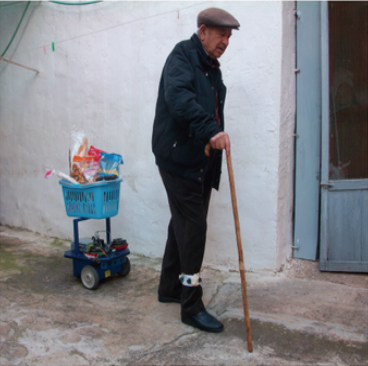
\includegraphics[width=0.4\textwidth]{figs/img/CompaRob}
   \caption{CompaRob robot~\cite{Sales2016-CompaRob}.}
   \label{fig:CompaRob}
 \end{figure}
% 
 Authors in~\cite{islam_lam_fukuda_kobayashi_kuno_2019} have developed a shopping
 support robot that employs a GRU (Gated Recurrent Unit) network to detect
 shopping habits of customers. The robot is also equipped with a LiDAR (Light
 Detection and Ranging) sensor and camera for detecting and building map of the
 customer's position using a two-dimensional skeleton and follow the customer
 through the store. The robot developed using such an algorithm is  shown in Fig.~\ref{fig:ShoppingSup}. %
%
\begin{figure}[htpb]
   \centering
   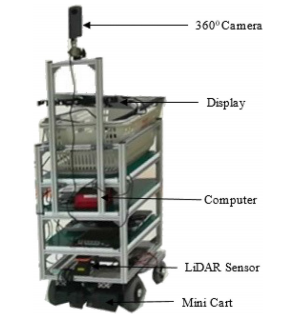
\includegraphics[width=0.35\textwidth]{figs/img/ShoppingSuportRobot}
   \caption{Shopping support robot.}
   \label{fig:ShoppingSup}
\end{figure}
%
Fig.~\ref{fig:SmartCart} shows a smart cart robot that has been developed by the authors in~\cite{Rawashdeh2017-Person}. The authors utilized an Arduino MEGA 2560, six
ultrasonic sensors, two DC motors with PWM (Pulse Width Modulation), an Android
Studio IDE device, and Bluetooth for detecting a customer and following them
through the store. %
%
\begin{figure}[htpb]
   \centering
   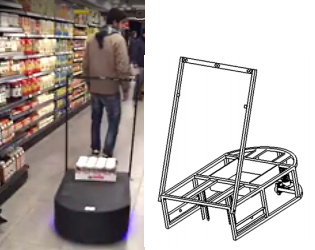
\includegraphics[width=0.40\textwidth]{figs/img/SmartCart}
   \caption{Smart Cart Robot}
   \label{fig:SmartCart}
\end{figure}
%
The operating principle of the proposed prototype of a smart robotic cart relies mainly on the radio frequency identification technology. For that, RF modules, XBee S2C RF radios, are primarily utilized to identify and communicate between the robotic cart and the remote (customer in a store, for example). XBee S2C RF radios are inexpensive and easily configurable. An RF module is configured as a remote target device that is carried
by the user/customer. The robot will be able to track this remote instead of using line
of sight methods~\cite{Miah2018-Intelligent}. In addition to the XBee S2C RF
radios, the robot is equipped with a parabolic reflector, which improves radio
reception at various distances and angles,~\textit{i.e.,} angle of arrivals of
RF signals from the remote, based on research done previously in this type of
robot localization and mapping~\cite{Miah2018-Intelligent,Li2013ANA}. The approach using signal strengths of RF signals also requires an understanding
of multipath interference which is common in RF based wireless positioning
sensing systems. Authors in~\cite{xie_jiang_zhao_zhang_2019} explain that using
course estimation calculations such as the received signal strength indicator (RSSI)
 together with the time difference of arrival (TDoA) is key to compensate for the effect of multipath
interference. 

The work in ~\cite{ladd_bekris_rudys_kavraki_wallach_2005} shows a different
approach to the multipath issue by using an IEEE 802.11b wireless Ethernet
device to measure RF signals. This device system was used because it is possible to communicate between a mobile device and a localization based service with low
complexity for the user. In~\cite{lindhe_johansson_bicchi_2007}, the research
states several other ways to counteract the multipath fading with methods such
as antenna diversity, frequency spreading, or adaptive antenna arrays. The
method used in this paper was to sample the radio signal strength (RSS) at
discrete points without too much deviation from the robot's desired position in
an indoor environment. Lastly, the method that is utilized in~\cite{Lindhe2009}
exploits multipath fading by measuring the signal-to-noise ratio (SNR) and
adjusting the robot's motion to spend more time where the channel strength is
greater. All solutions reported in the literature referred to here required line-of-sight
communication between the robot and the user. However, in this work, we aim to use the
XBee S2C RF radios and a parabolic reflectors integrated into a rotating system
similar to the one presented in~\cite{Miah2018-Intelligent} in order to have the
robot track the customer through a store without using line-of-sight sensing.
The major challenge of this implementation is the estimation of the distance
between the robot and the remote in various operating environments.



\section{System Architecture}
\label{sec:systemArchitecture}
The proposed smart robotic cart is a wheeled mobile robot that sends and
receives radio signals to follow the remote target (customer in a store, for
example) which acts as a beacon. The high-level system block diagram of the
proposed robotic cart (prototype) is shown in Fig.~\ref{fig:sys_block_diag}. %
% 
\begin{figure}[htbp]
  \centering
  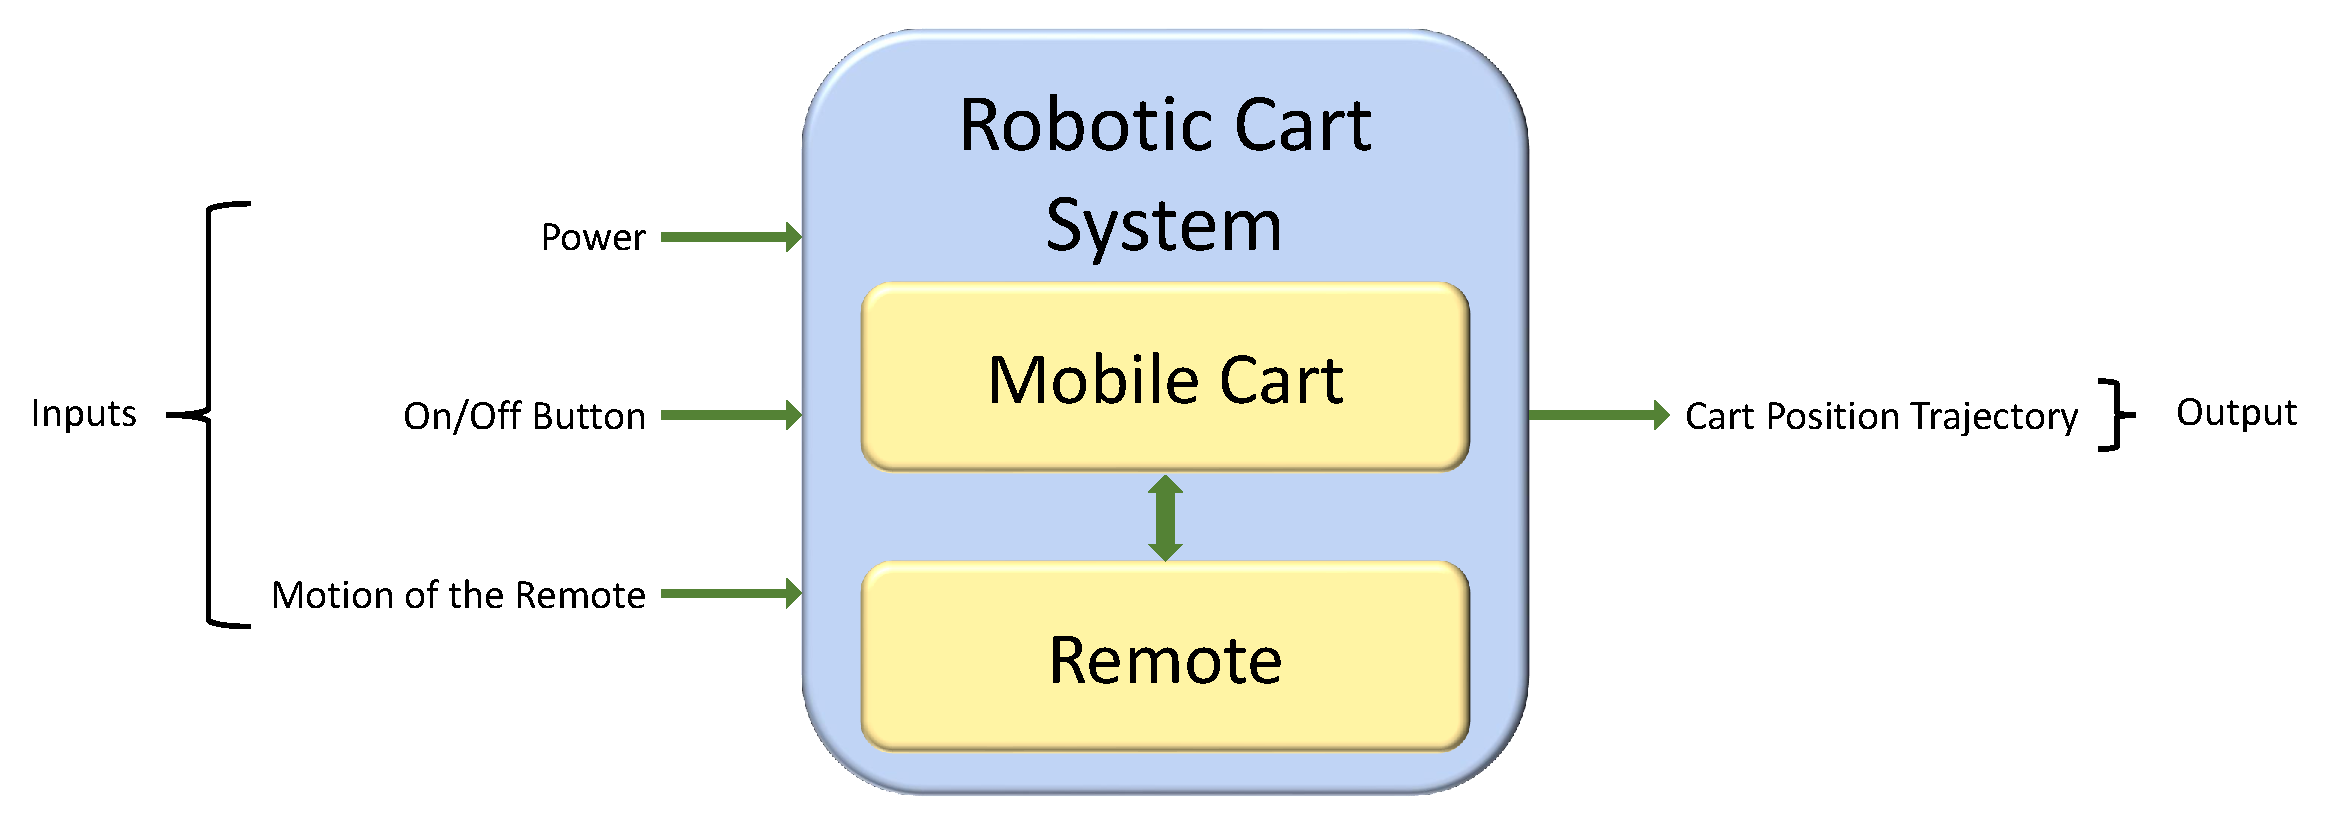
\includegraphics[width=0.5\textwidth]{figs/systemBlockDiagram.pdf}
  \caption{System level block diagram detailing inputs and outputs to the
    robotic cart system.}
	\label{fig:sys_block_diag}
\end{figure}
% 
There are three inputs to the proposed cart system. The robotic cart is supplied
with power through a battery that is mounted in the chassis of the robotic cart.
There will be an on/off switch to allow the cart to be powered down when not in
use. This will save the battery from being drained by other electronic
components of the robot. The motion of the robotic cart is dependent on the
motion of the remote. The main output of the system is the position trajectory
of the robotic cart in its environment. When the user/customer moves with the
remote target, the robotic cart is designed to follow the user.

As can be seen, two subsystems (mobile cart and remote) of the proposed robotic cart communicate with one another by relaying radio messages between them. Fig.~\ref{fig:remote_block_diag} shows the block diagram of the remote. %
%
\begin{figure}[htbp]
  \begin{subfigure}[b]{0.9\linewidth}
    \centering
    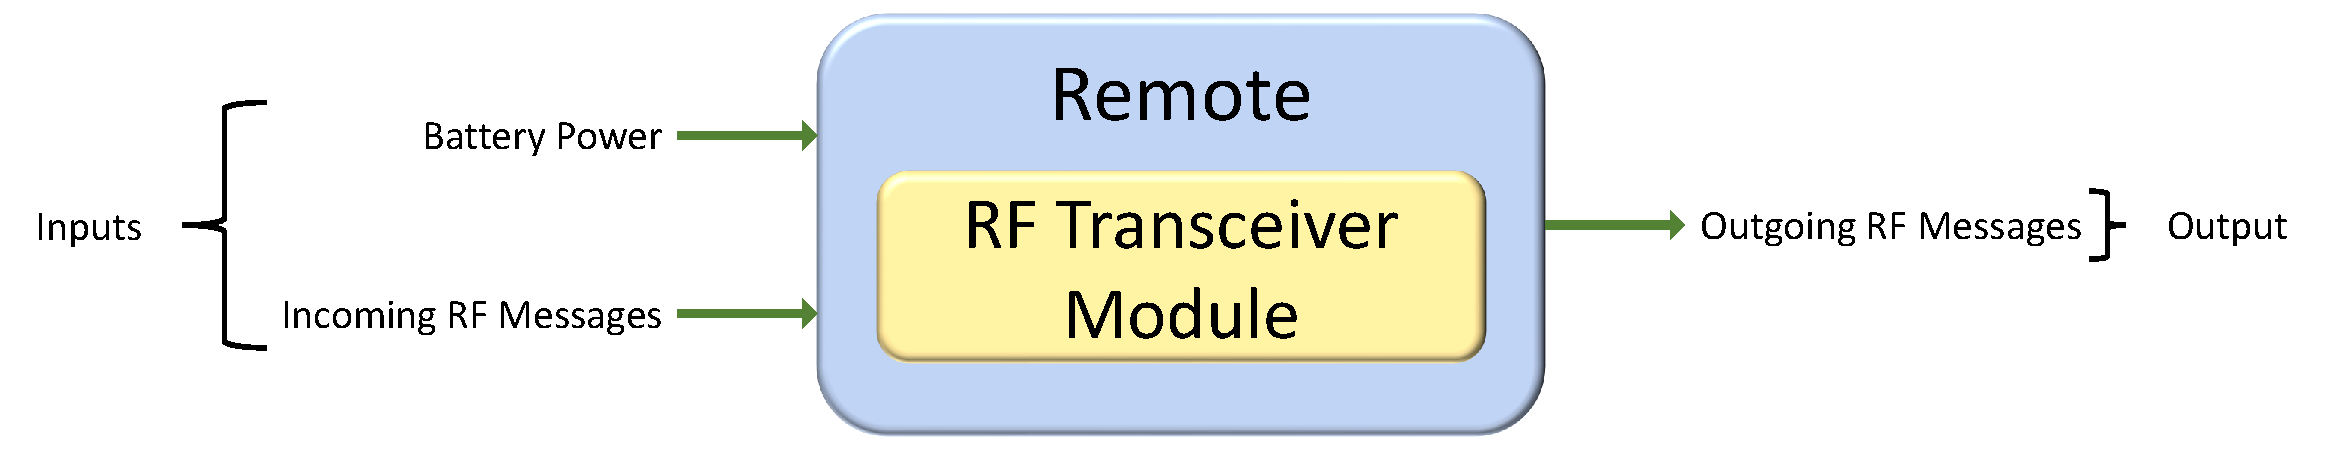
\includegraphics[width=\textwidth]{figs/remoteBlockDiagram.pdf}
    \caption{}
    \label{fig:remote_block_diag}
  \end{subfigure}
  \begin{subfigure}[b]{0.9\linewidth}
    \centering
    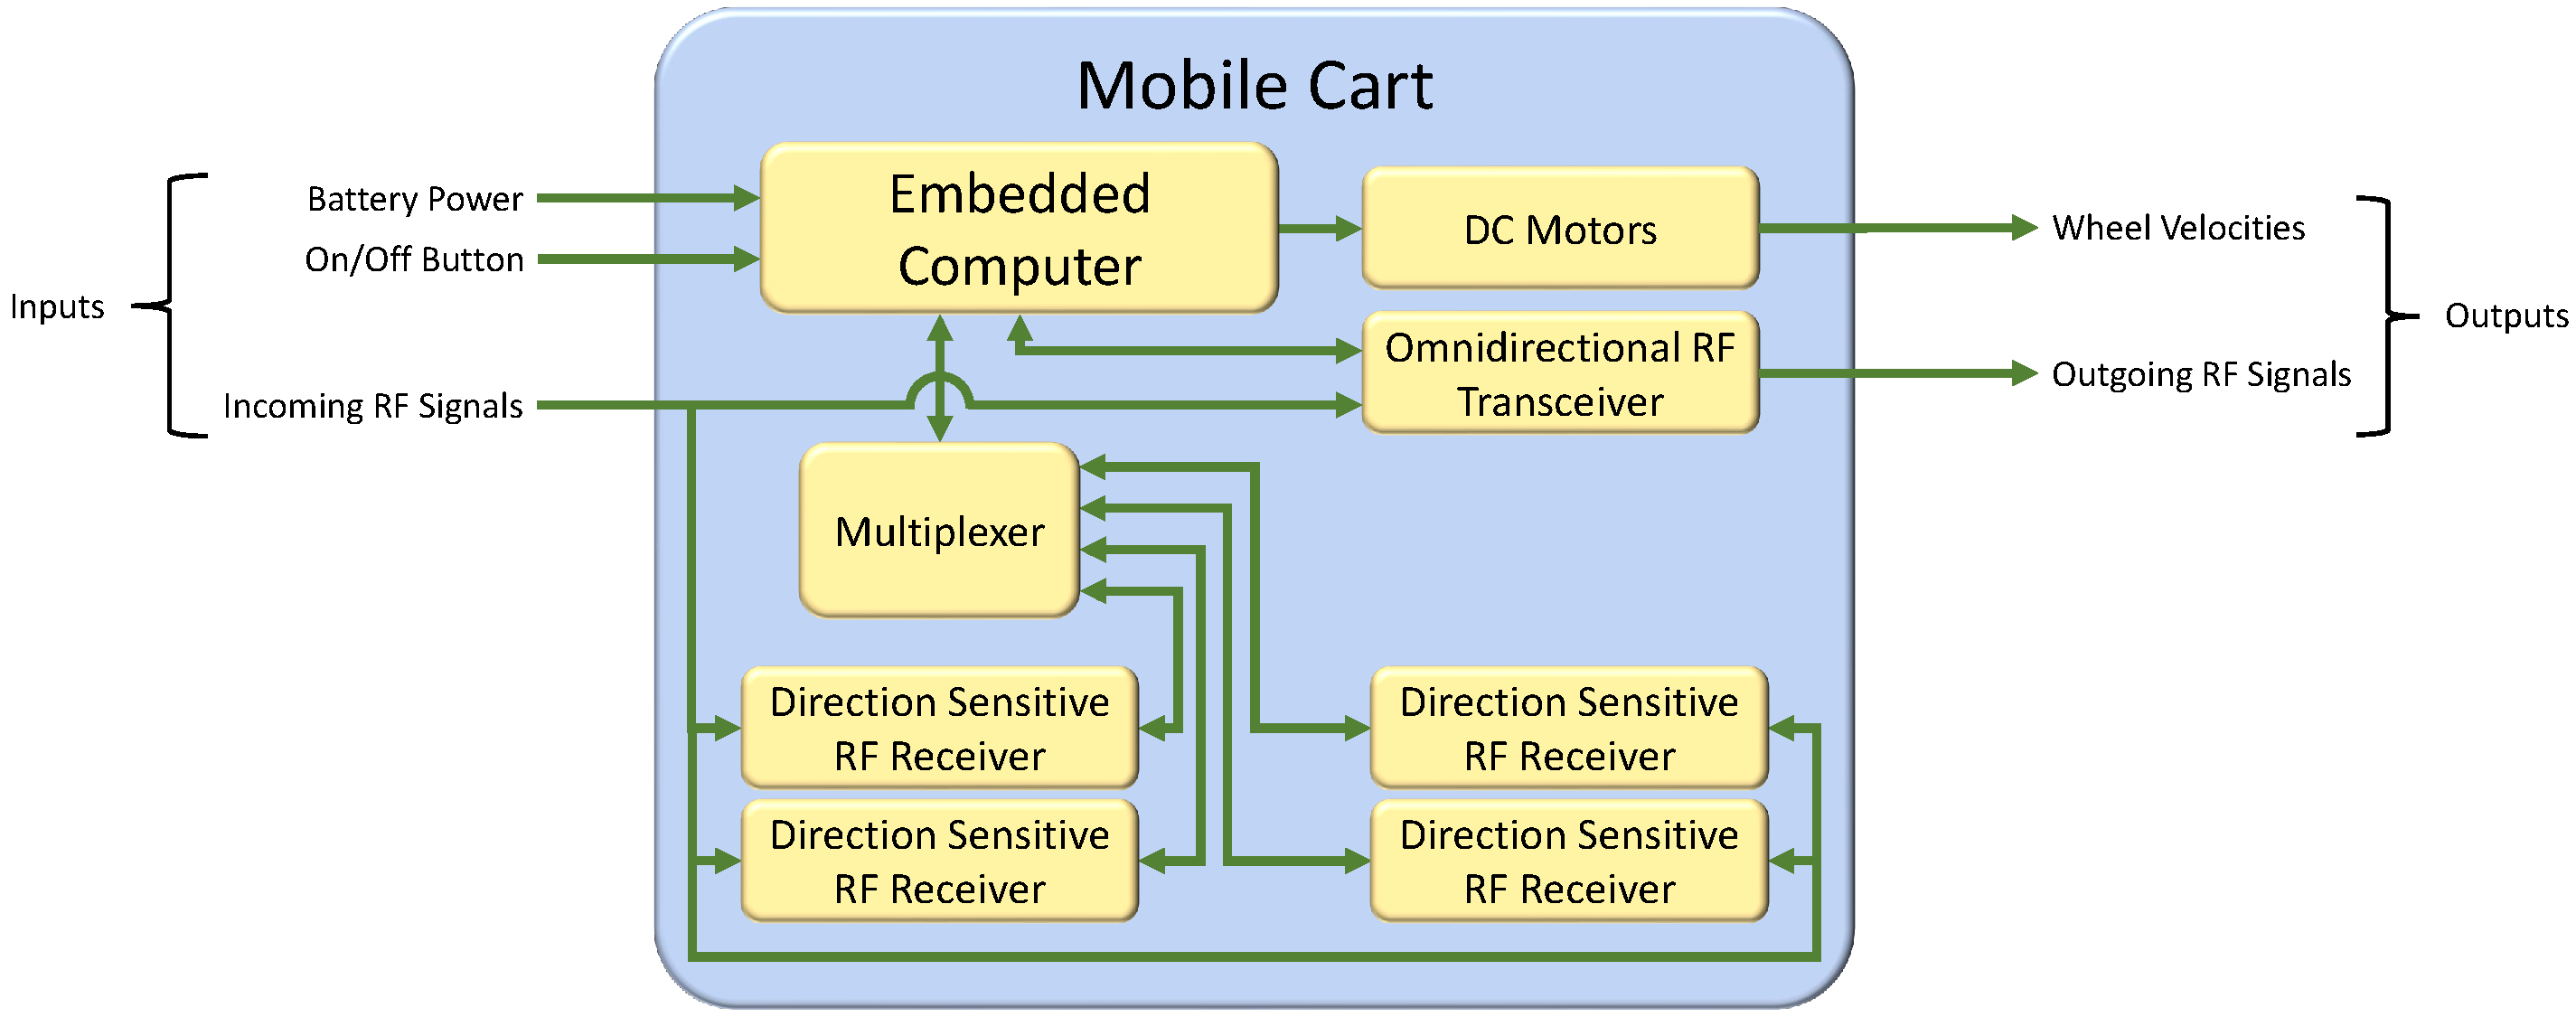
\includegraphics[width=\textwidth]{figs/mobileCartBlockDiagram.pdf}
    \caption{}
    \label{fig:mobile_block_diag}
  \end{subfigure}
  \caption{Block diagrams showing inputs and outputs of:~\subref{fig:remote_block_diag} remote and~\subref{fig:mobile_block_diag}~mobile cart of the proposed smart robotic cart.}
  \label{fig:blockDiagramRemoteMobileCart}
\end{figure}
%
It requires an RF module, XBee, attached to $7.4~[\si{\volt}]$ Li-Po battery
with a voltage regulation circuit since the XBee has a smaller input voltage of
$3.3~[\si{\volt}].$ The two inputs of the remote are the battery power and the
incoming RF messages which are passed through the RF transceiver. The remote
outputs the RF message back to the mobile cart, which will be discussed
later. The subsystem block diagram of the mobile cart is shown in
Fig.~\ref{fig:mobile_block_diag}. The cart requires a power source, which will
be a $7.4~[\si{\volt}],$ $8000~[\si{\milli\ampere\hour}]$ Li-Po battery since the Li-Po works well with powering the
embedded computer. The power to the subsystem will be toggled
by an on/off switch located on the chassis of the robotic cart. The final input
to the mobile cart subsystem are the incoming RF signals and the wheel velocities for the cart's actuators. These incoming RF
signals are passed to the direction sensitive RF receivers which output the
signals to the dual-direction multiplexer. The dual-direction multiplexer then
takes the four inputs from the direction sensitive RF receivers and passes one
output into the embedded computer. Once the embedded computer gets these signals
it can apply localization and navigation algorithms and pass the necessary actuator commands to the actuators of the robotic cart. 



%----------------------------------------------------------------------
\section{Main Construction Components}
\label{sec:mainConstructionComponents}
%----------------------------------------------------------------------

There are several components that are required for constructing the proposed
smart robotic cart. The main components are the Budget Bot Chassis
(Fig.~\ref{fig:budgetBotChassis}), the BeagleBone Blue embedded robotics
computer (Fig.~\ref{fig:beagleboneBlue}), and the XBee S2C RF modules
(Fig.~\ref{fig:xbeemodule}). %
%
\begin{figure}[htbp]
  \centering
  \begin{subfigure}[b]{0.3\linewidth}
    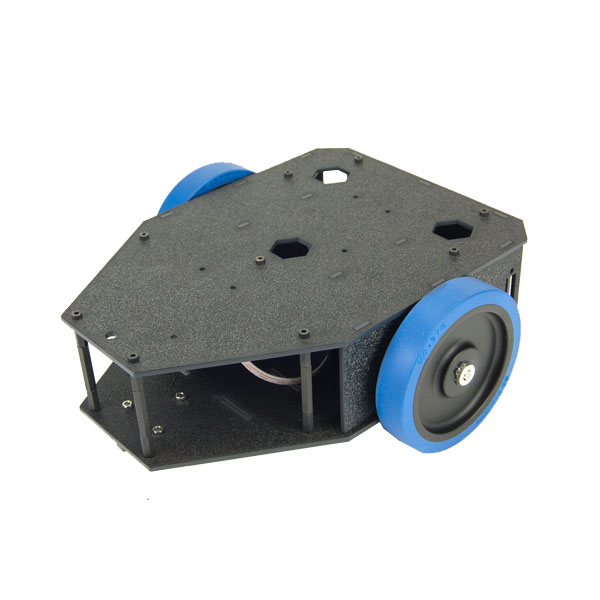
\includegraphics[width=1\textwidth]{figs/img/budgetbot_chassis}
    \caption{}
    \label{fig:budgetBotChassis}
  \end{subfigure}
  \begin{subfigure}[b]{0.3\linewidth}
    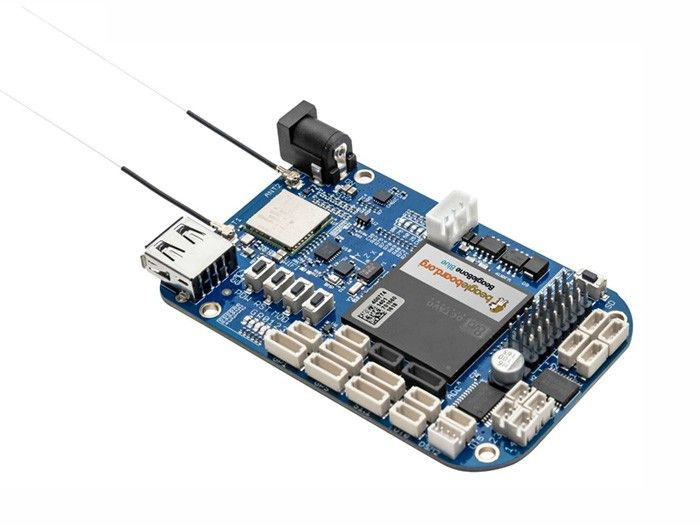
\includegraphics[width=1\textwidth]{figs/img/beaglebone_blue}
    \caption{}
    \label{fig:beagleboneBlue}
  \end{subfigure}
  \begin{subfigure}[b]{0.3\linewidth}
    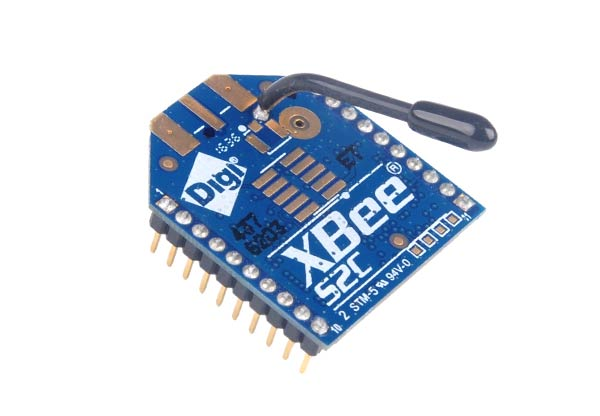
\includegraphics[width=1\textwidth]{figs/img/Xbee-S2C-Module}
    \caption{}
    \label{fig:xbeemodule}
  \end{subfigure}
  \caption{The main components for constructing the proposed smart robotic cart:~\subref{fig:budgetBotChassis} Budget Bot robot chassis, ~\subref{fig:beagleboneBlue} BeagleBone Blue embedded robotics computer, and~\subref{fig:xbeemodule} XBee S2C RF module.}
\end{figure}
%
Note that the radiation pattern of XBee RF modules is omnidirectional. However,
it is desired to have differences in the signals received by the RF modules
mounted on the robot based on the angle from which the signal is coming from the
remote. Therefore, one of the major components of the robotic cart is the
reflector array that enables the XBee modules to be direction sensitive.

\subsection{Reflector Array Design}
\label{sec:reflectorArrayDesign}
Two different models of reflector arrays were designed and constructed (see Fig.~\ref{fig:reflectorDesigns}). %
%
\begin{figure}[htbp]
  \centering
  \begin{subfigure}[b]{0.45\linewidth}
    \centering
    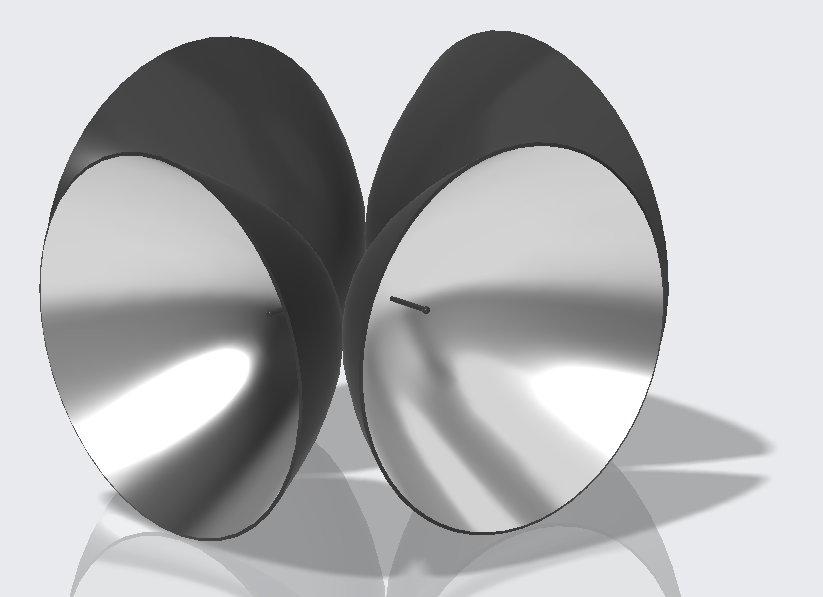
\includegraphics[width=\textwidth]{figs/img/paraboloidalReflector.png}
    \caption{}
    \label{fig:paraboloidalReflector}
  \end{subfigure}
  \begin{subfigure}[b]{0.45\linewidth}
    \centering
    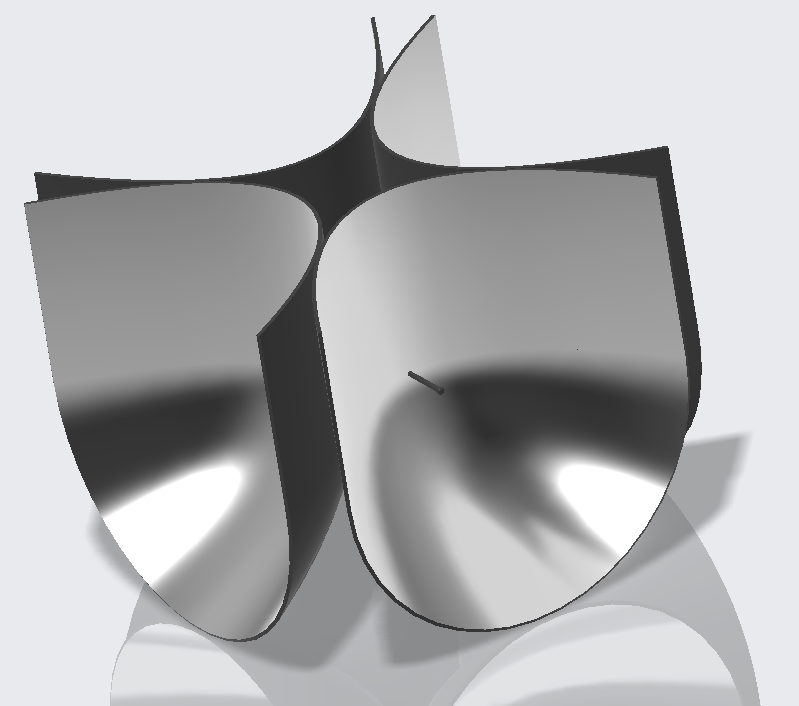
\includegraphics[width=\textwidth]{figs/img/parabolicReflector.png}
    \caption{}
    \label{fig:parabolicReflector}
  \end{subfigure}
  \caption[Reflector designs]{Two different reflector design for the robotic cart:~\subref{fig:paraboloidalReflector} Purely paraboloidal reflector array~and~\subref{fig:parabolicReflector} parabolic/paraboloidal reflector array.}
  \label{fig:reflectorDesigns}
\end{figure}
%

The first design, shown in Fig.~\ref{fig:paraboloidalReflector}, uses a
reflector with a paraboloidal shape. This shape was selected since all signals
entering the reflector parallel to the axis of the reflector will be focused at
the focal point of the paraboloid. By mounting the XBee such that the center of
the antenna coincides with the focal point of the paraboloid, the signal
strength of the signals entering parallel to the axis will be maximized. The
second design, shown in Fig.~\ref{fig:parabolicReflector}, is the same on the
lower half as the first design. However, the upper half is simply a surface
where the horizontal cross-section is a parabola. The purpose for this design is
similar to that of the first design, but the parabolic shape on the top will
allow stronger detected signal strength of signals coming from above the
reflector. Since the remote will be held by a person, it will generally be above
the robot. The parabolic/paraboloidal reflector design is intended to allow
better reception of signals from above.


\subsection{Reflector Construction}
With the recent advancements in 3D printing technology, it is not difficult to
create an object with a parabolic shape. Here, the reflector dishes
were created using a 3D printer. The reflector array was designed to be modular,
where the dishes, top plate, and bottom frame were printed separately. After
printing, the dishes were lined with foil tape to provide the reflective surface
to focus the signals onto the antenna of the XBee. A layer of foil tape was also
placed on the top plate to provide a ground plane for the XBee. The parts were
then fastened together using M3 screws and nuts (see Fig.
\ref{fig:reflectorConstruction}).
%
\begin{figure}[htbp]
    \centering
    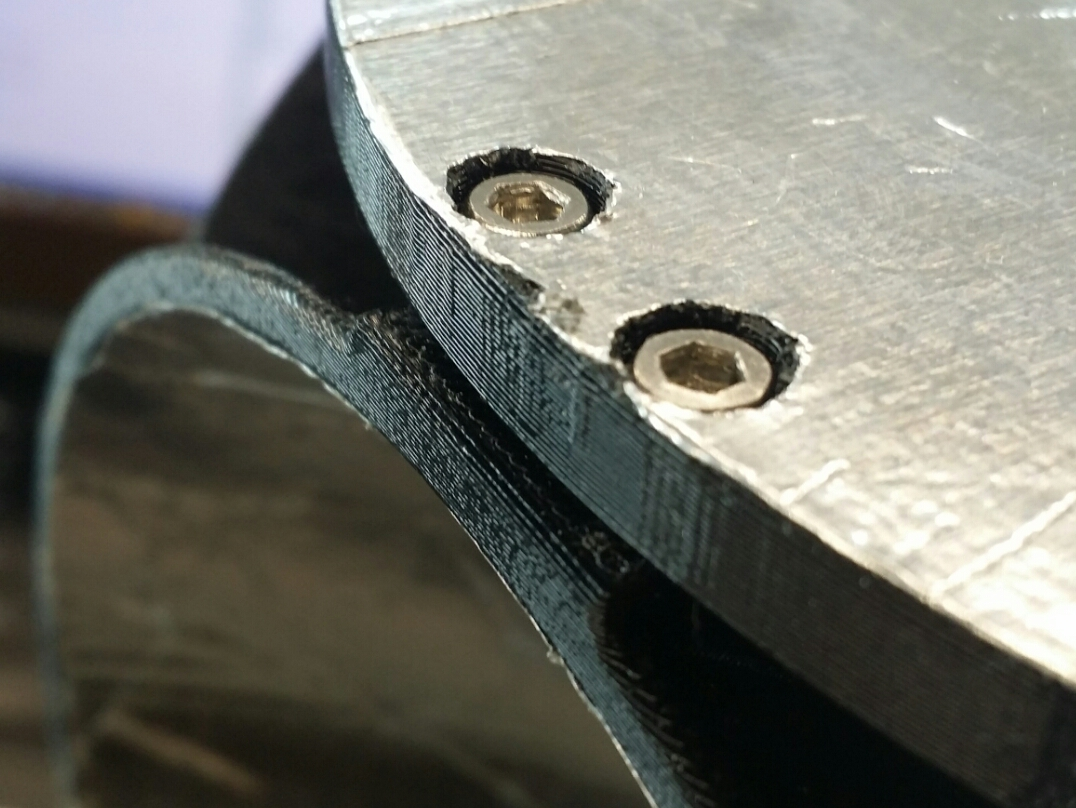
\includegraphics[scale=0.1]{figs/img/reflectorConstruction.jpg}
    \caption{Reflector construction using 3D printer.}
    \label{fig:reflectorConstruction}
\end{figure}
%


% ----------------------------------------------------------------------
\section{Localization and Navigation}
\label{sec:locAndNavAlgos}
%----------------------------------------------------------------------

This section illustrates the localization and navigation algorithms for the
proposed robotic cart to operate in an indoor/outdoor environment. For the sake
of simplicity, the cart is modeled as a differential drive mobile robot (DDMR).
The direction and distance of the remote relative to the cart are determined
using a localization algorithm. The estimated distance and angle are then passed
to a navigation algorithm which calculates and applies the actuator commands
(in this case, wheel speeds of the robot) to move the robot toward the remote.

\subsection{Robot Model}\label{subsec:robotModel}
The robot used in this work was a differential drive mobile robot, which has
two drive wheels and a caster wheel for the balance. The robot turns by applying
different speeds to the left and right wheels. As shown in Fig.~\ref{fig:robotGeometry}, the radius of the wheels is $R$, and the distance
between the wheels is $L.$ The pose of the robot is given by the $x$-coordinate
($x$), the $y$-coordinate ($y$), and the orientation, ($\theta$), as shown in
Fig.~\ref{fig:robotPose}. %
%
\begin{figure}[htbp]
    \centering
    \begin{subfigure}{0.4\linewidth}
        \centering
        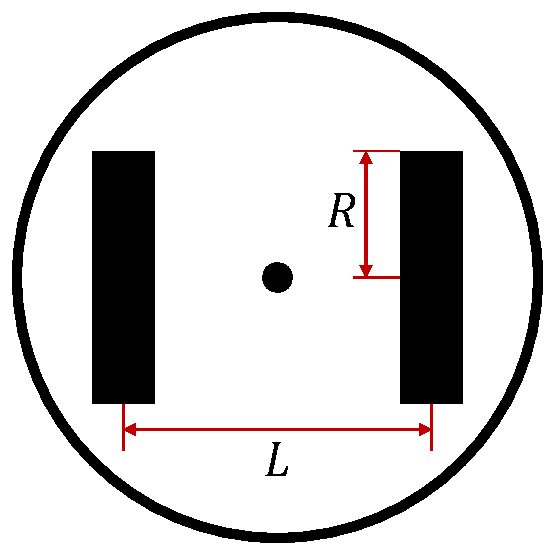
\includegraphics[width=\textwidth]{figs/robotGeometry.pdf}
        \caption{}
        \label{fig:robotGeometry}
    \end{subfigure}%
    \begin{subfigure}{0.4\linewidth}
        \centering
        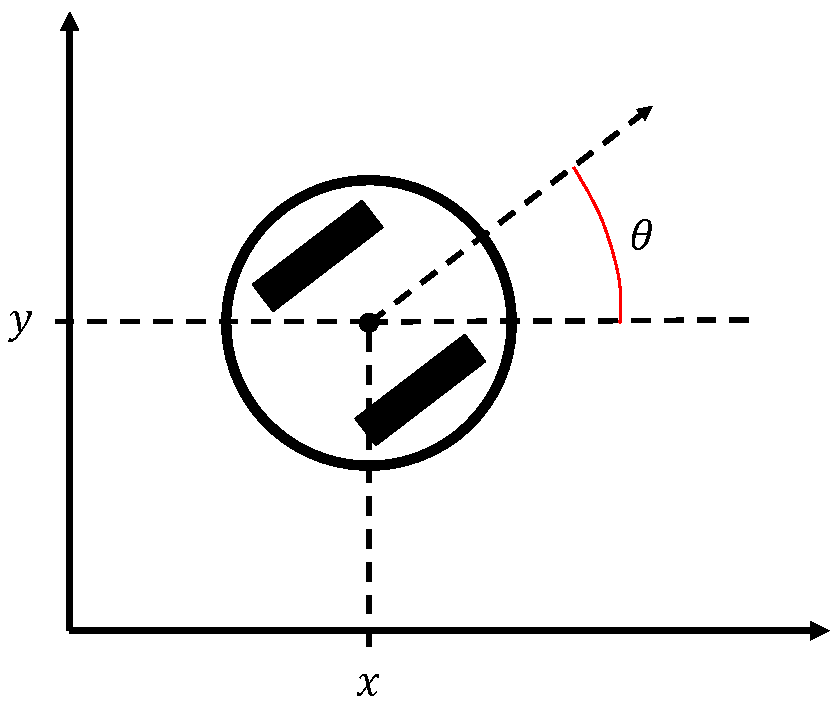
\includegraphics[width=\textwidth]{figs/robotPose.pdf}
        \caption{}
        \label{fig:robotPose}
    \end{subfigure}
    \caption{Kinematics of the robotic cart modeled as a DDMR.}
    \label{fig:robotModelParameters}
\end{figure}
%
Generally, the robot is controlled by commanding a linear and angular speed ($v$ and $\omega$, respectively). These speeds are converted into left and right wheel speeds. The following equations are used to calculate the angular left and right wheel speeds ($\omega_l$ and $\omega_r$, respectively): %
%
\begin{align*}
  \omega_l = \left(v - \omega\frac{L}{2}\right)\frac{1}{R}\qq{and} \omega_r = \left(v + \omega\frac{L}{2}\right)\frac{1}{R}.
\end{align*}
%
To control DC motors in this way, the relationship between duty cycle and angular speed must be determined. Then the duty cycles to apply to the wheels can be calculated for the commanded $v$ and $\omega$.

\subsection{Relative Localization of Remote}
The localization algorithm is used to estimate the position of the remote with
respect to the mobile robot/cart's local coordinate frame. First, the omnidirectional
transceiver mounted on top of the reflectors sends a signal strength request to the
remote. The remote then replies with a message containing the strength of the
signal it just received. This reply is detected by the receivers inside the
reflectors as well as the omnidirectional transceiver. The strength detected by
each of the directional receivers and the strength contained in the reply are
then recorded. At this point, the entire reflector array is rotated
$\ang{9},$ and this process is repeated. The robot continues taking
measurements in this way until the reflectors have been rotated one quarter
turn. Since there are four reflectors at $\ang{90}$ to each other, a strength
measurement has been recorded for every $\ang{9}$ increment around the robot.
The angle of the remote is then estimated as the direction from which the
strongest signal was received. The distance to the remote is calculated using
the free-space path loss formula. The direction of reflector rotation is then
reversed since the wires connecting the RF modules in the reflectors prevent the
reflector from freely spinning. A flowchart of this algorithm is shown in Fig.~\ref{fig:localizationAlgoFlowchart}. %
%
\begin{figure}[htbp]
    \centering
    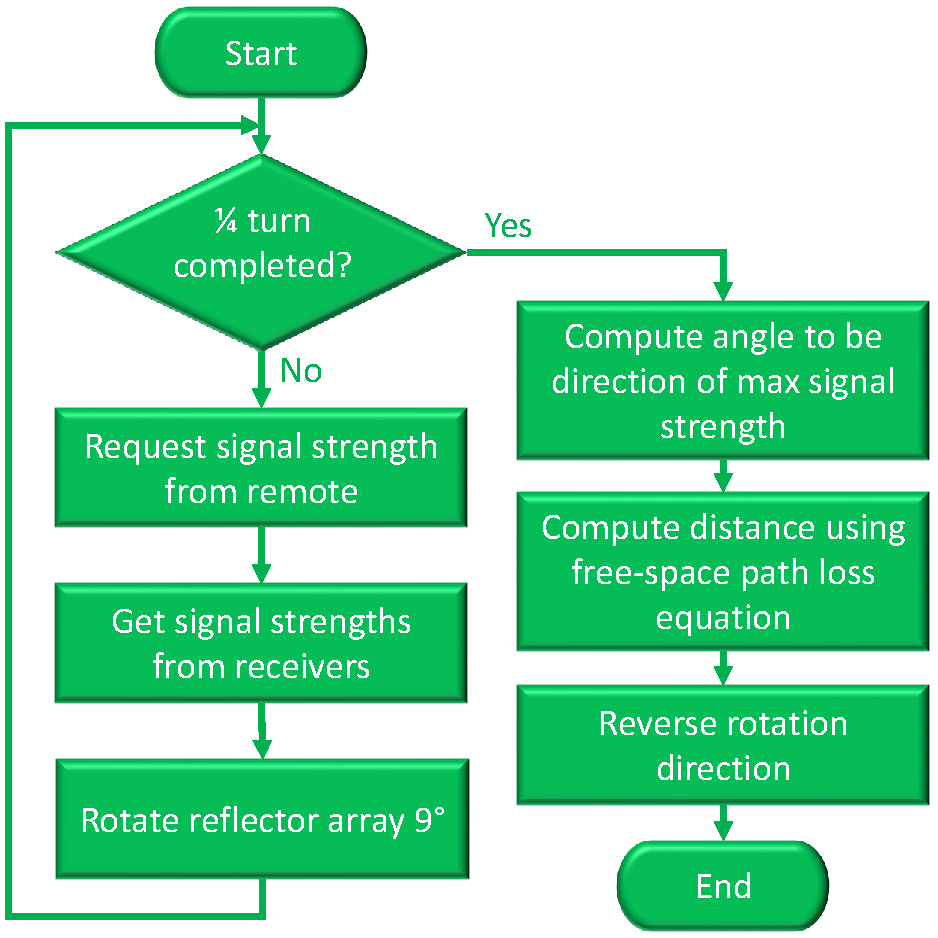
\includegraphics[width=.48\textwidth]{figs/localizationAlgorithmFlowchart.pdf}
    \caption{Flowchart localizing the remote.}
    \label{fig:localizationAlgoFlowchart}
\end{figure}

\subsection{Navigation of Mobile Cart}\label{subsec:navAlgo}
The navigation algorithm is used to drive the robot toward the remote. The inputs to the navigation algorithm are the angle to the remote ($\theta_r$) and the distance to the remote ($d_r$). A target point is then calculated as the point that is in the same direction as the remote, but closer to the robot by a fixed following distance ($d_{follow}$), as shown in Fig.~\ref{fig:navAlgoDiagram}. The distance to the target point is calculated as $d_{tgt} = d_r - d_{follow}$, and the angle to the target point is $\theta_{tgt} = \theta_r$. The linear and angular speeds of the robot ($v$ and $\omega$, respectively) are then calculated using proportional control by the following equations: %
%
\begin{align*}
  v = K_vd_{tgt}\qq{and}\omega = K_\omega\theta_{tgt}.
\end{align*}
%
The appropriate duty cycles are then calculated as specified in section~\ref{subsec:robotModel} and applied to the wheel DC motors (robot actuators). %
%
\begin{figure}[htbp]
    \centering
    \begin{subfigure}{0.45\linewidth}
        \centering
        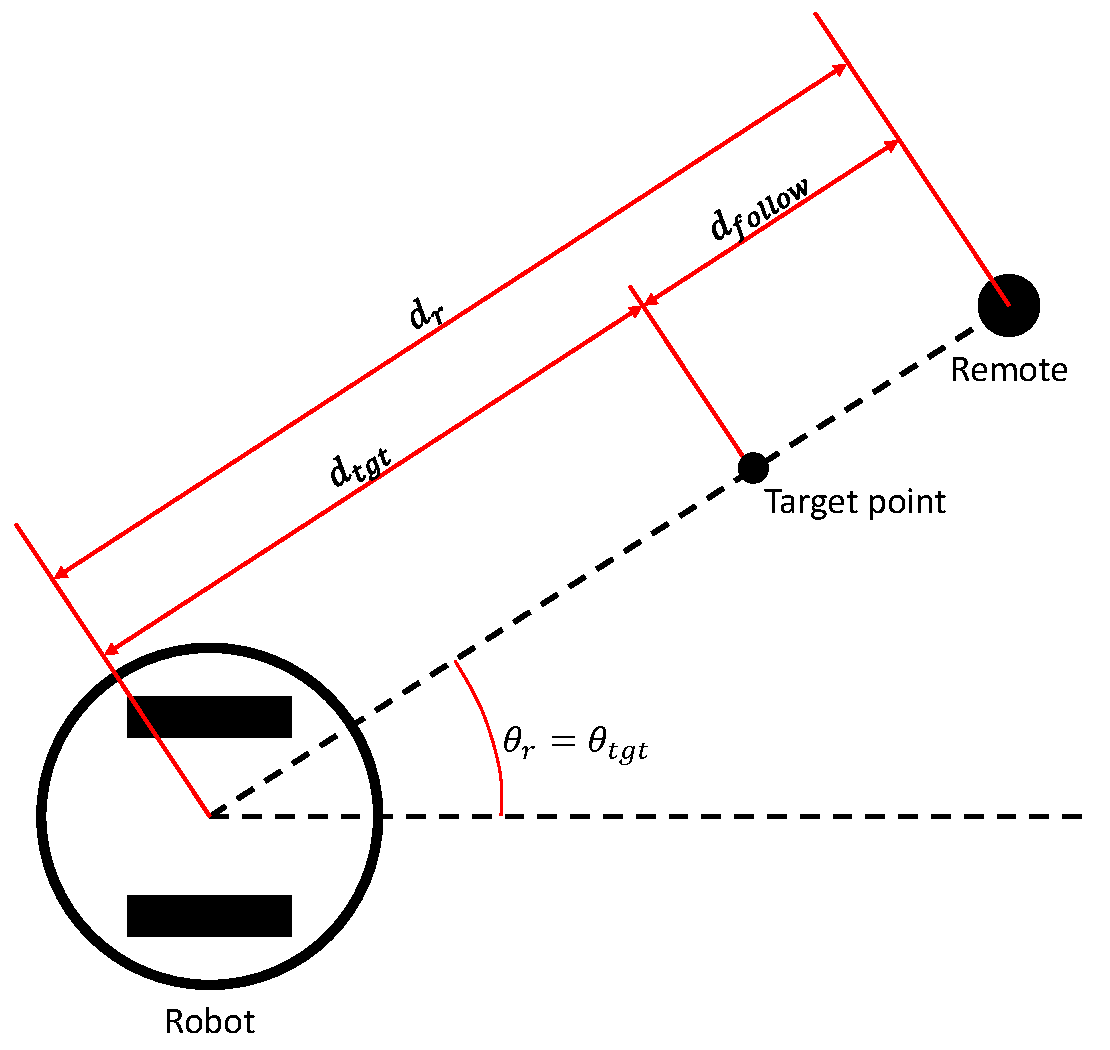
\includegraphics[width=\textwidth]{figs/navigationAlgorithmDiagram.pdf}
        \caption{Target Point Diagram}
        \label{fig:navAlgoDiagram}
    \end{subfigure}%
    \begin{subfigure}{0.45\linewidth}
        \centering
        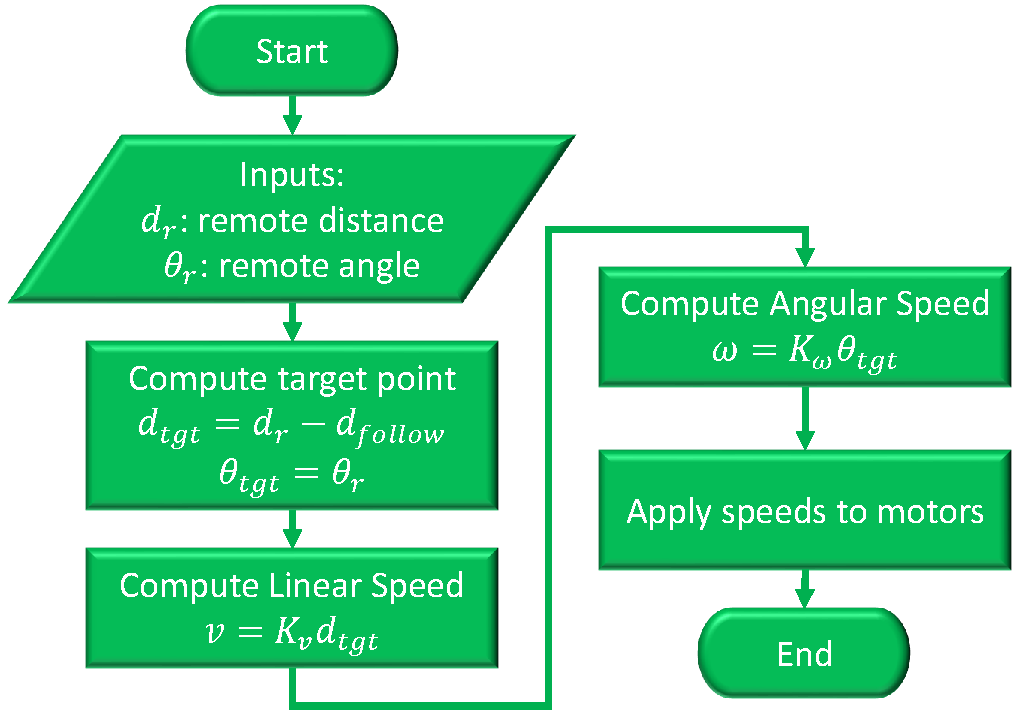
\includegraphics[width=\textwidth]{figs/navigationAlgorithmFlowchart.pdf}
        \caption{Flowchart}
        \label{fig:navAlgoFlowchart}
    \end{subfigure}
    \caption{Navigation algorithm for the mobile cart to move towards the remote.}
    \label{fig:navAlgoDetails}
\end{figure}


\section{Hardware Implementation and Prototype}
\label{sec:hardwareImplementation}



The remote and mobile cart were designed and implemented using off-the-shelf
components. A customized Budget Bot chassis was the base of the proposed smart
robotic cart. The new DC motors installed in the Budget Bot are Pololu 27D Metal
Gear motors which provide a max speed of $2.72~[\si{\meter\per\second}]$ when
using the wheels with a diameter of $2R = 98~[\si{\milli\meter}].$ These motors
allow the robotic cart to follow the remote that can move at an average person's
walking speed. The next step was to attach the BeagleBone Blue microcomputer,
XBee reflector array assembly, and breadboard to the top of the robot. A 2-cell
LiPo battery was also installed inside the chassis of the mobile cart to provide
power to the BeagleBone Blue directly and the breadboard through the
switch. %The power supplied to the breadboard is sent through a regulator circuit to drop it down from the 7.4V of the LiPo to 3.3V of the XBee. This circuit is also used on the remote which consists of a 7.4V LiPo battery and the XBee module with voltage regulator in between. This voltage regulator is built out of a LM117 regulator and a 10uF ceramic capacitor between the input and output pins of the regulator. %
The circuit diagrams for the robot and remote are shown in Figs.
\ref{fig:robotCircuit} and \ref{fig:remoteCircuit}. %

\begin{figure}[htbp]
  \centering
  \begin{subfigure}[b]{0.47\linewidth}
    \centering
    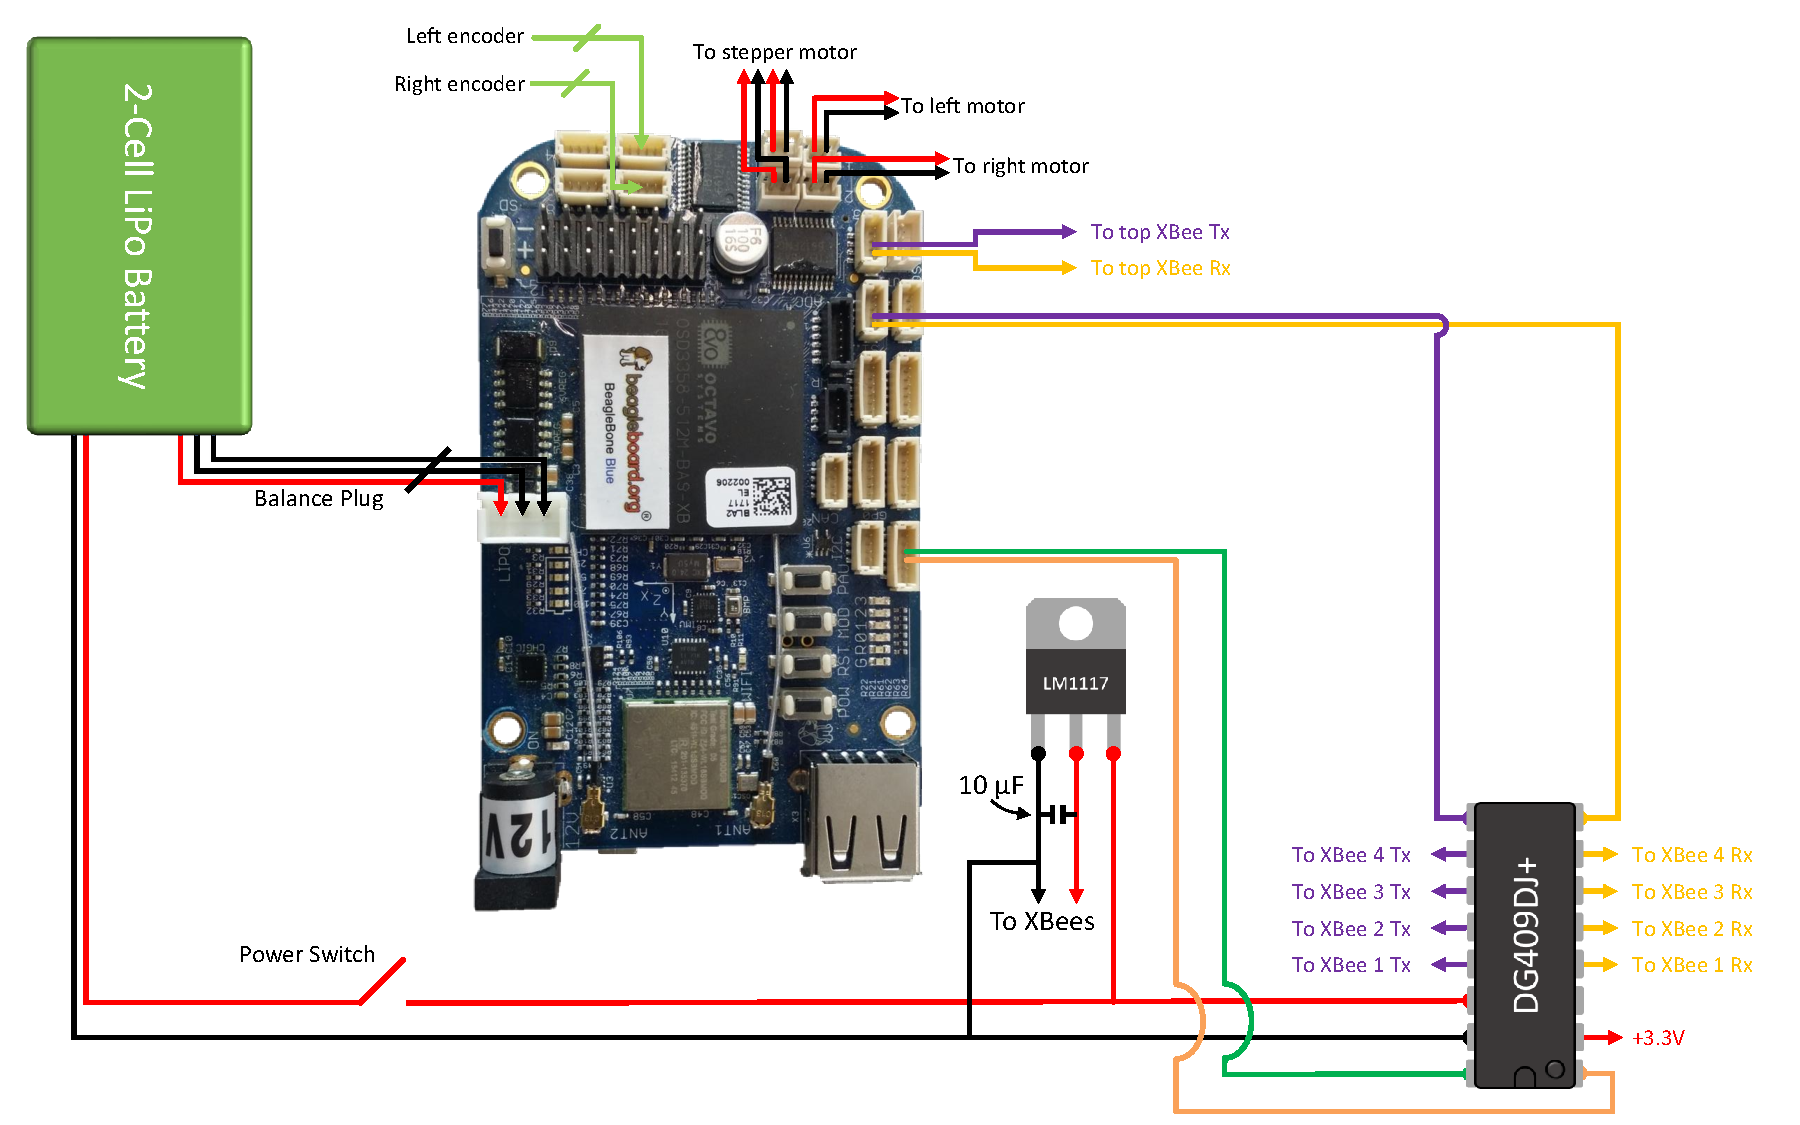
\includegraphics[width=\textwidth]{figs/robotCircuit.pdf}
    \caption{}
    \label{fig:robotCircuit}
  \end{subfigure}
  \begin{subfigure}[b]{0.47\linewidth}
    \centering
    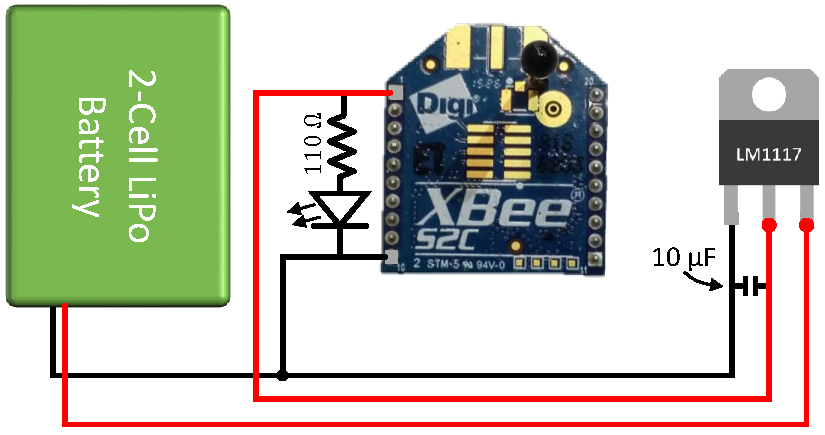
\includegraphics[width=\textwidth]{figs/remoteCircuit.pdf}
    \caption{}
    \label{fig:remoteCircuit}
  \end{subfigure}
    \caption{Circuit diagrams for~\subref{fig:robotCircuit} robotic cart~and~\subref{fig:remoteCircuit} remote.}
    \label{fig:CktDiagramRoboticCartRemote}
\end{figure}
%
The reflector array  was mounted on a stepper motor that was then attached to a 3D printed bracket. This bracket was then attached to the chassis using M3 screws. Another feature of this bracket is that it had a stop block built into the top  to allow the robot to automatically initialize the reflector array to the zero position when the robot starts up. This is accomplished by commanding a turn of \ang{90} and allowing the reflectors to hit the stop block and be held there until this turn is complete. %
The Xbee modules from the reflector array posed a bit of a problem when it came to connecting them to the BeagleBone Blue. The BeagleBone Blue has three standard UART ports and two others found in the USB and UART-GPS, which makes a total of five UARTs. Unfortunately, not all five ports can be used to communicate with XBees since UART0 is used to provide communication with a computer through the console. Since port 0 is reserved for this function, the number of usable ports is only four, but the robot requires communication with five XBees. The solution to this problem was to use two of the GPIO pins, two of the UART ports, and a dual 4-channel multiplexer. One of the UARTs can be directly connected to the top XBee, and the other UART can be routed through the multiplexer to the four side XBee modules. Then two UART ports are used to communicate with all five XBees. %
The complete prototype of the proposed robotic cart and remote are shown in Fig.~\ref{fig:finishedPrototypes}. %
%
\begin{figure}[htbp]
    \centering
    \begin{subfigure}[b]{0.4\linewidth}
        \centering
        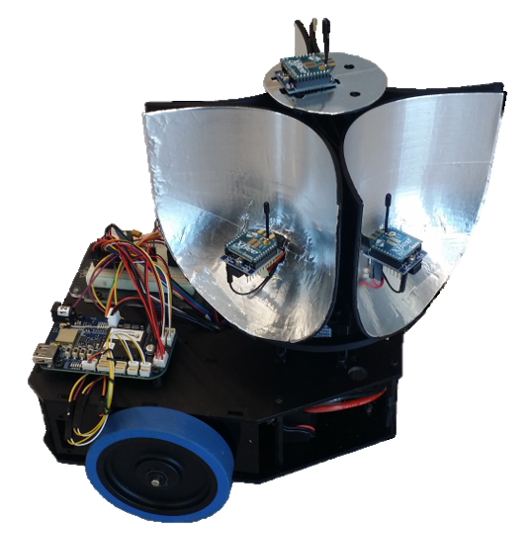
\includegraphics[width=\textwidth]{figs/img/Finalized_robot.png}
        \caption{}
        \label{fig:overallPrototype}
    \end{subfigure}
    \begin{subfigure}[b]{0.4\linewidth}
        \centering
        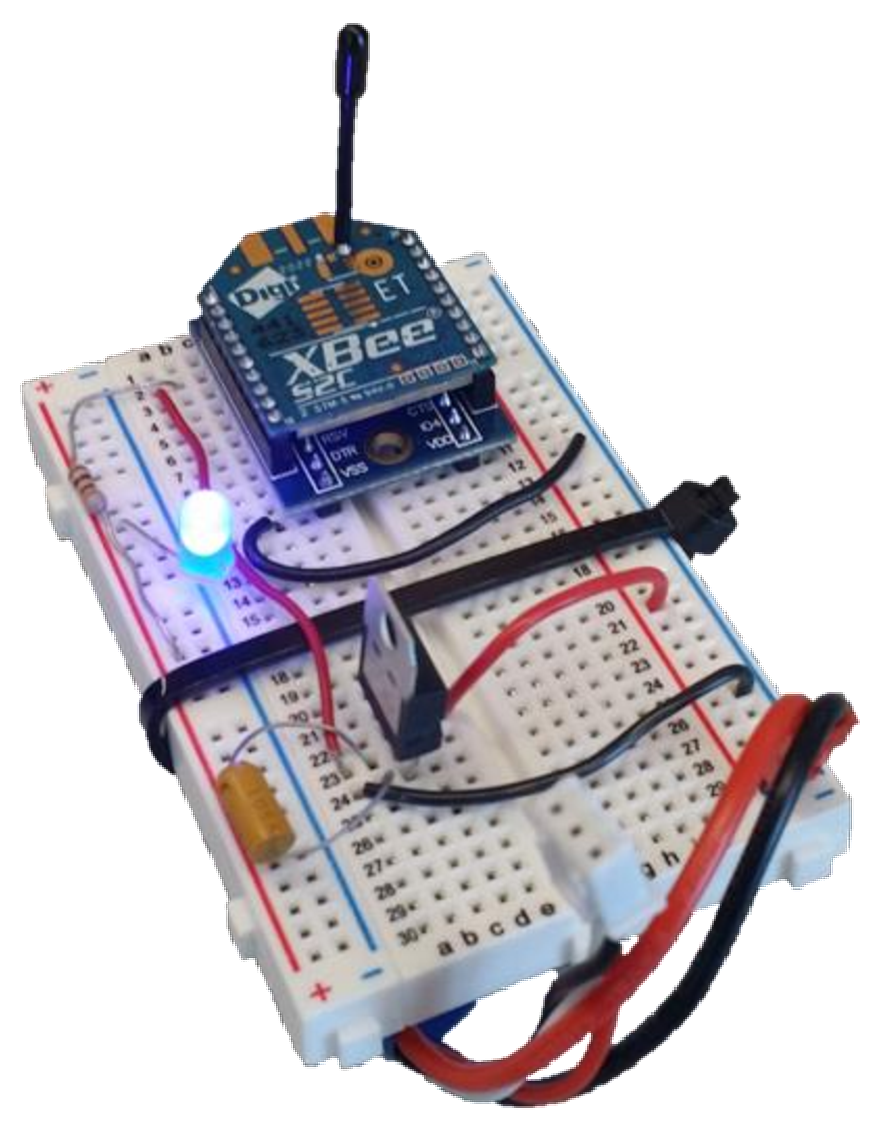
\includegraphics[scale=0.25]{figs/remote.pdf}
        \caption{}
        \label{fig:remotePrototype}
    \end{subfigure}
    \caption{The complete prototype of the proposed smart robotic cart~\subref{fig:overallPrototype} mobile robotic cart~and~\subref{fig:remotePrototype} remote.}
    \label{fig:finishedPrototypes}
\end{figure}
%
The BeagleBone Blue embedded robotics computer already has a set of ports on it
that can be accessed and controlled using the Robot Control Library from
Strawson Design (see
\href{http://strawsondesign.com/docs/librobotcontrol/}{http://strawsondesign.com/docs/librobotcontrol/},
for details). Some custom libraries were built on top of the robot control
library to handle XBee frames, AT commands, and the stepper motor control. The
XBee Frames library takes a given block of data containing the message and then
packages it into a XBee frame to send over UART to the XBee desired module. The
XBee communications library also handles received messages from the XBee module
and validates the received frame's integrity and extracts the message data from
it. On top of the XBee communications library there is a library that generates
AT Commands to package in the XBee frames. The AT command library also handles
extracting response data from the AT response command structure and validates
it. See the process for XBee communication over UART in
Fig.~\ref{fig:CommandProcessDiagram}. %
%
\begin{figure}[htbp]
  \centering
  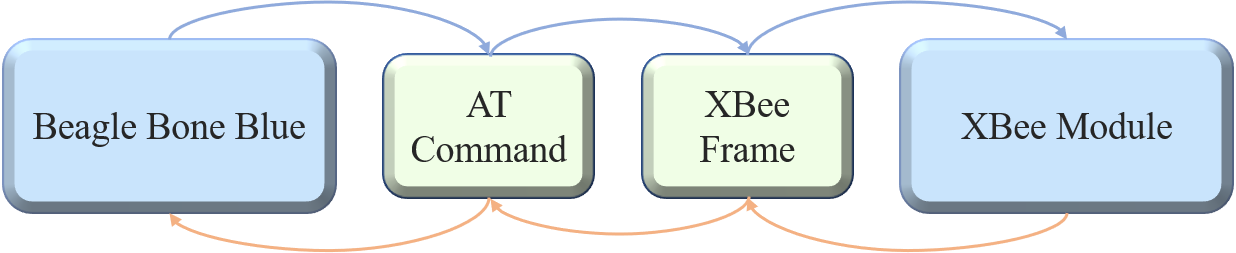
\includegraphics[width=0.48\textwidth]{figs/img/Command Process Diagram.png}
  \caption{Process for XBee communication over UART.}
  \label{fig:CommandProcessDiagram}
\end{figure}
%
The final custom library is the stepper motor control library. This library had
to be written since instead of using a dedicated stepper motor controller, two
of the regular BBBlue DC motor control ports were used to power the stepper
motor. The library handled translating how many steps to turn into the phase
states to be sent to the DC motor ports that are connected to the stepper motor.
The library also helped to keep track of basic information related to the
stepper motor such as what its current angle should be.

%----------------------------------------------------------------------
\section{Experimental Results}
\label{sec:Experimental Results}
%----------------------------------------------------------------------

After the robotic cart and the remote were built, several different variants of
the algorithms were tested. There were two main types of variants tested. In one
variant, the stepper motor is locked, preventing the reflector from rotating. In
the other variant, the stepper motor is used to sweep through the angles. The
experiments with the complete prototype of the proposed smart robotic cart shown
in Fig.~\ref{fig:finishedPrototypes} were conducted on a hallway, a laboratory
floor, and the ground floor of the Business and Engineering Convergence Center
of Bradley University. %
%
\begin{figure}[htbp]
  \centering
  \begin{subfigure}[b]{0.30\linewidth}
    \centering
    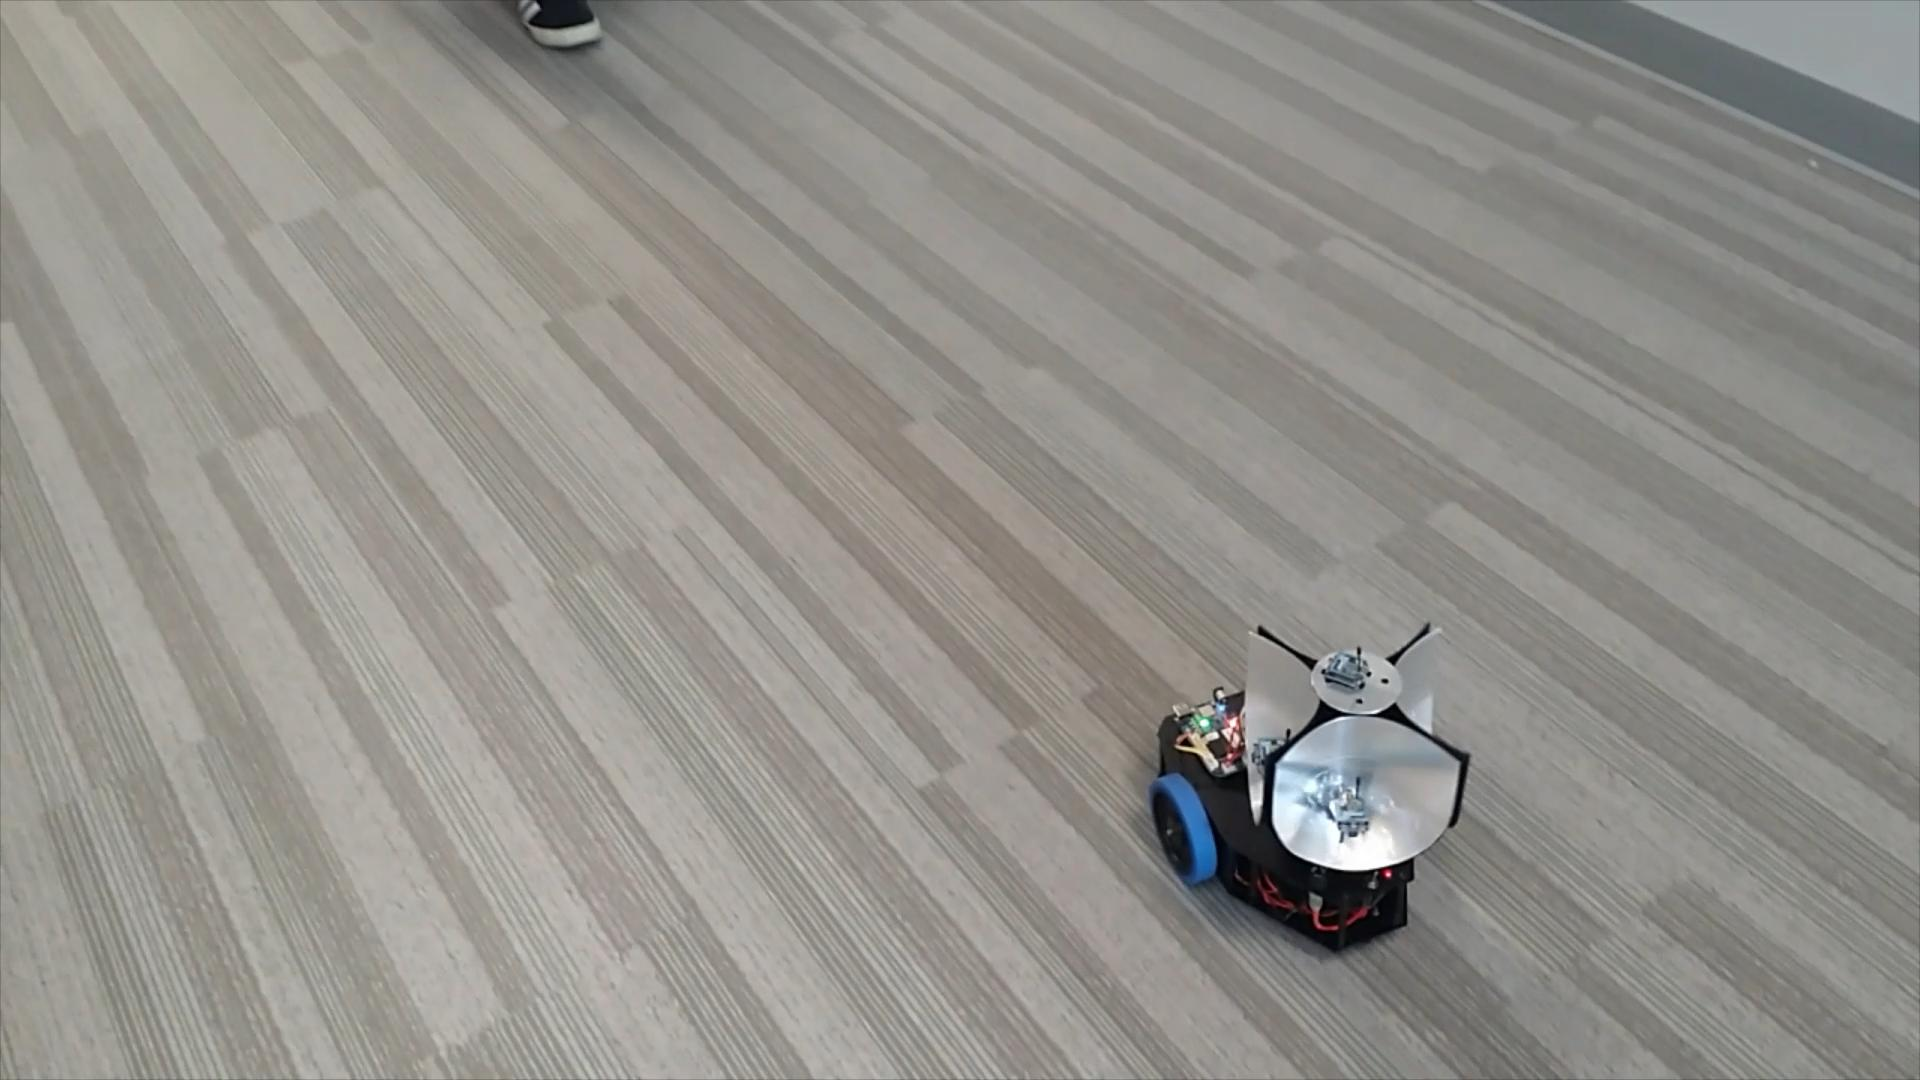
\includegraphics[width=\textwidth]{videos/frames/71.jpeg} 
    \caption{}
    \label{fig:71}
  \end{subfigure}
  \begin{subfigure}[b]{0.30\linewidth}
    \centering
    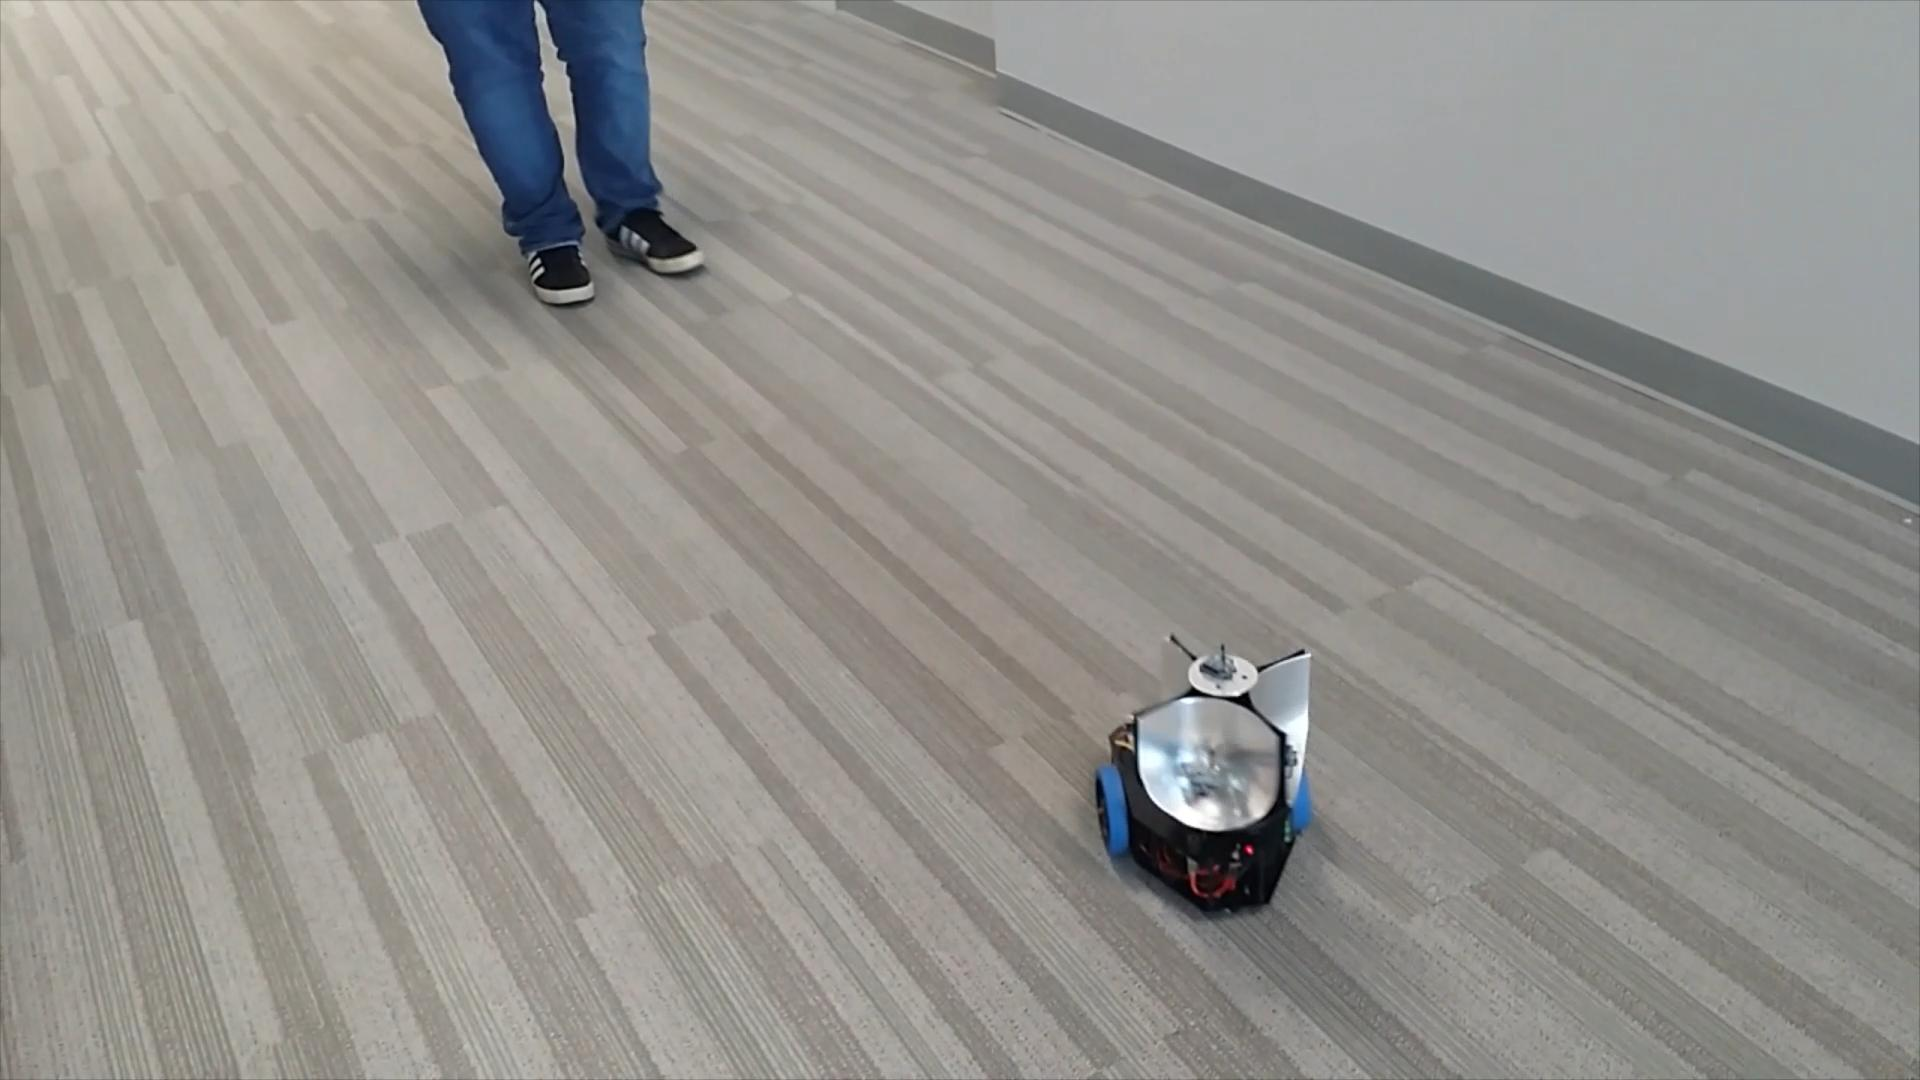
\includegraphics[width=\textwidth]{videos/frames/141.jpeg} 
    \caption{}
    \label{fig:141}
  \end{subfigure}
  \begin{subfigure}[b]{0.30\linewidth}
   \centering
   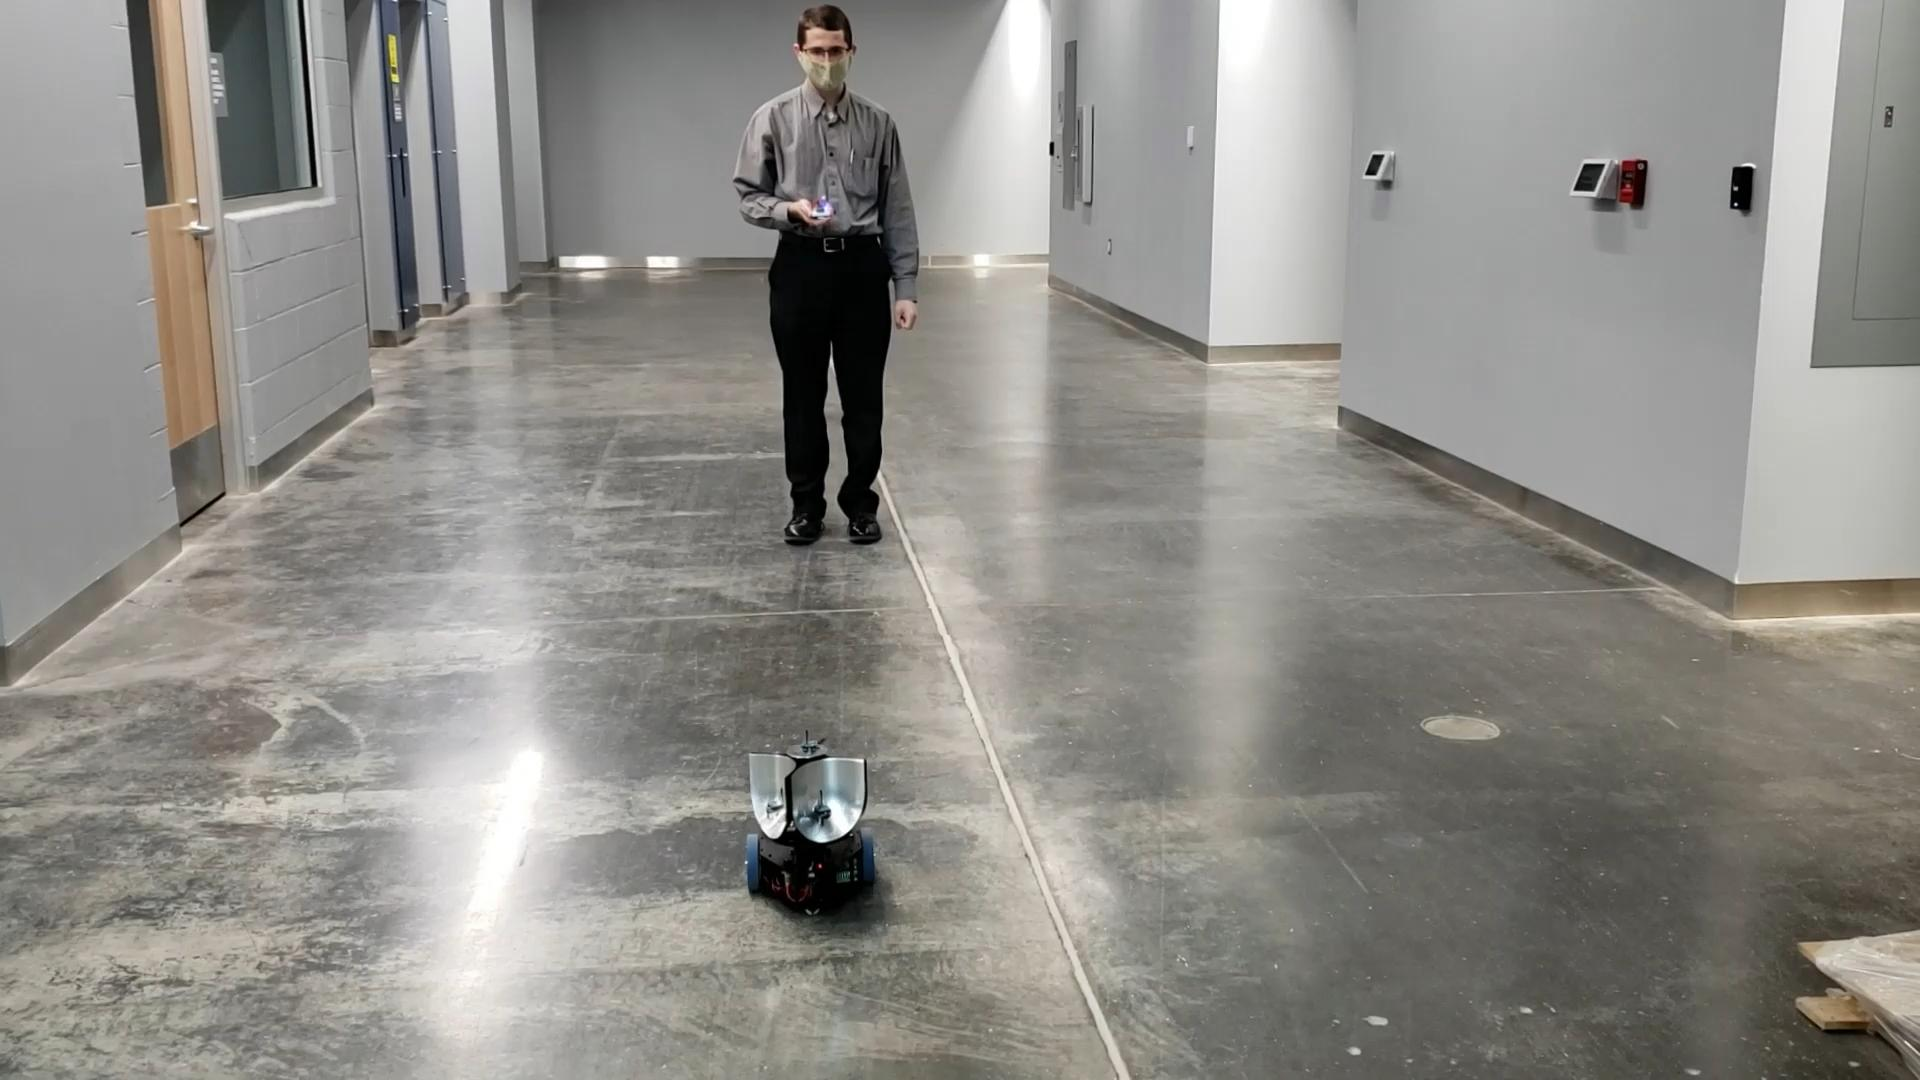
\includegraphics[width=\textwidth]{videos/frames/211.jpeg} 
   \caption{}
   \label{fig:211}
 \end{subfigure}
 \\
  \begin{subfigure}[b]{0.30\linewidth}
    \centering
    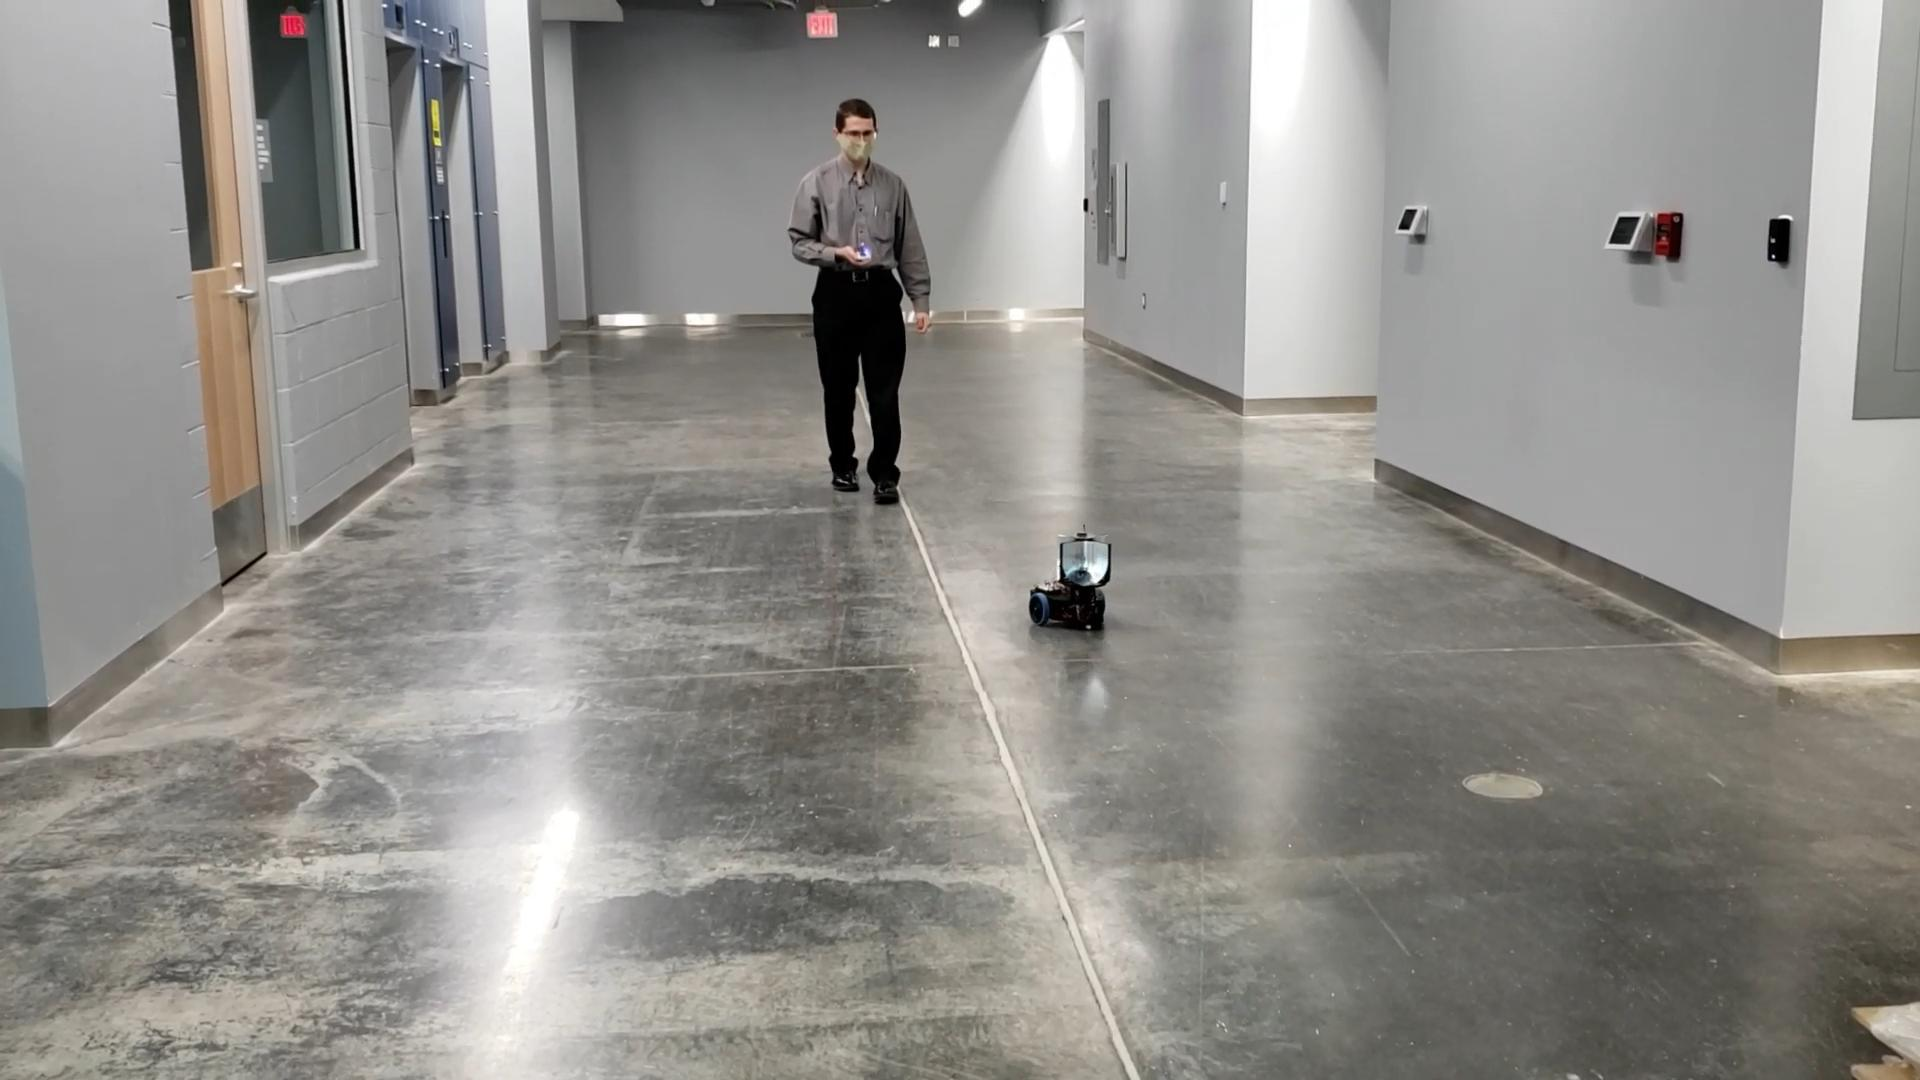
\includegraphics[width=\textwidth]{videos/frames/351.jpeg} 
    \caption{}
    \label{fig:351}
  \end{subfigure}
  \begin{subfigure}[b]{0.30\linewidth}
    \centering
    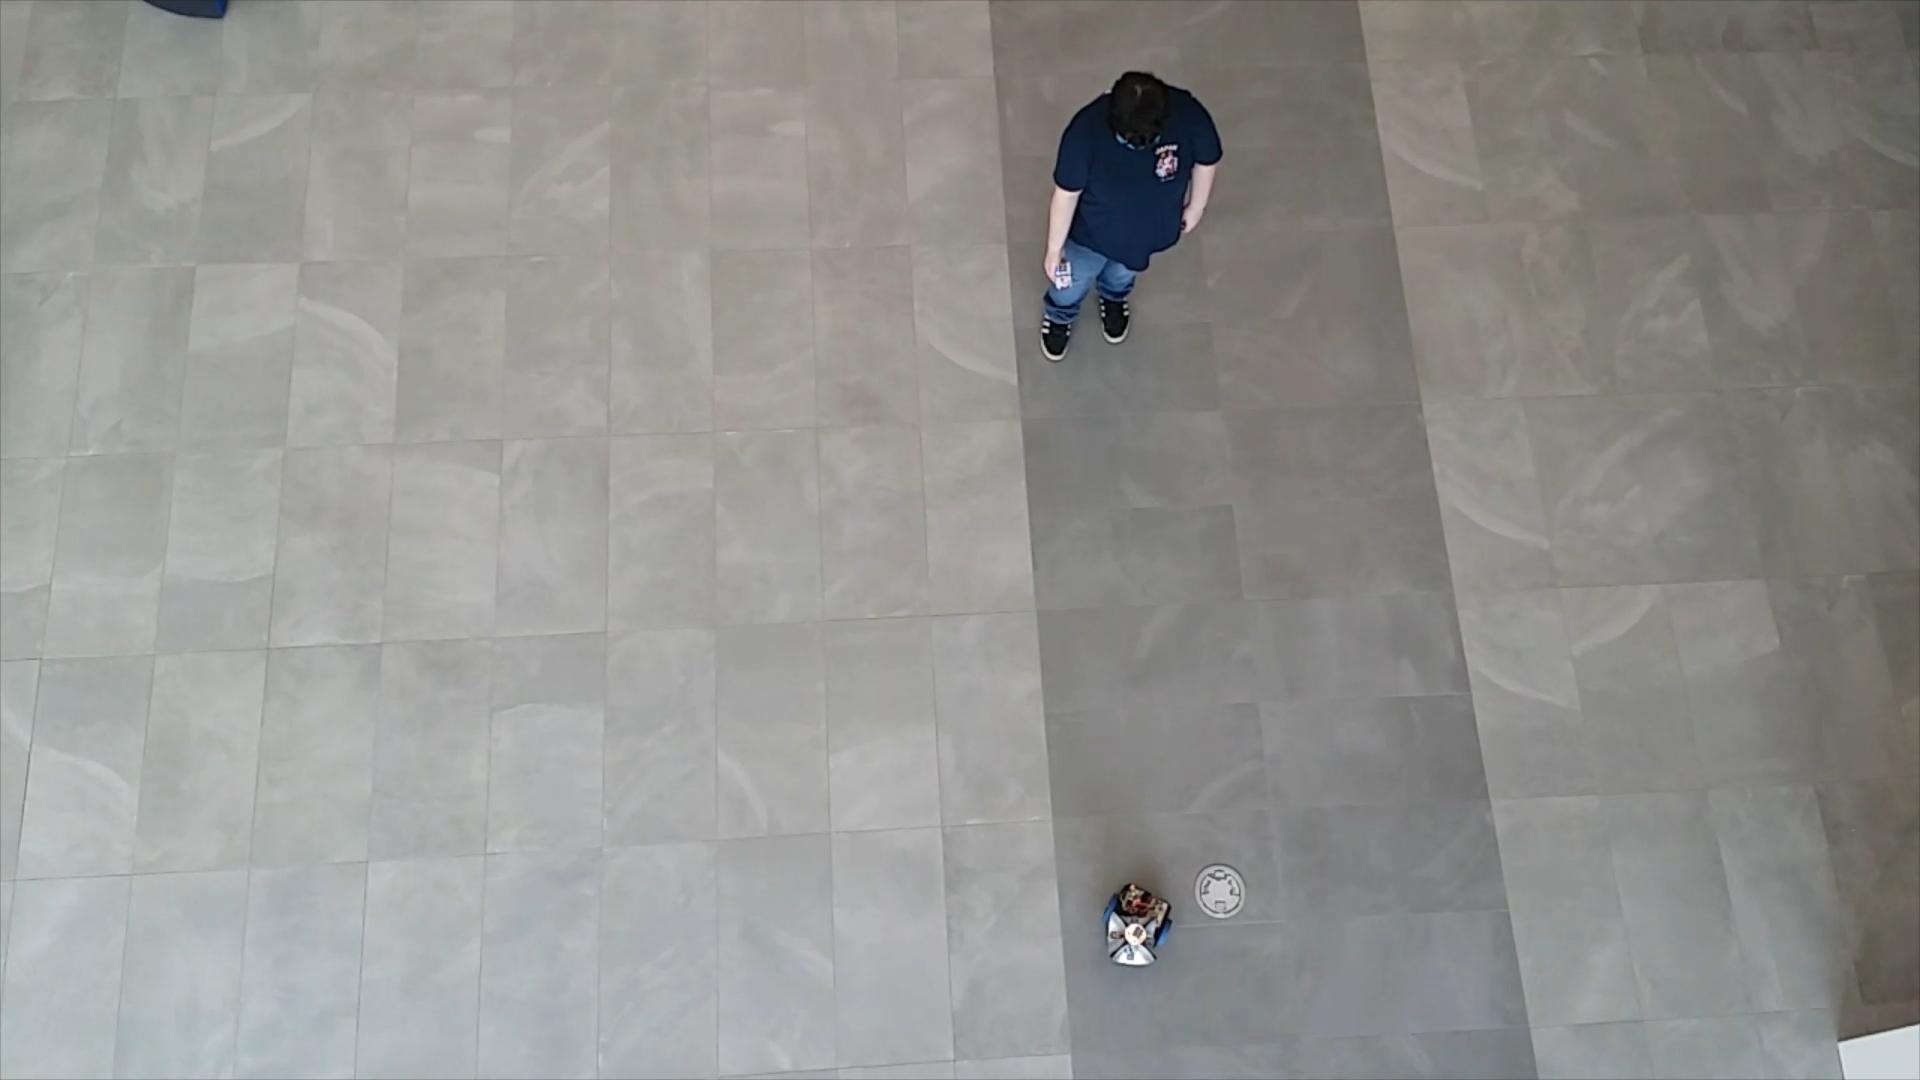
\includegraphics[width=\textwidth]{videos/frames/491.jpeg} 
    \caption{}
    \label{fig:491}
  \end{subfigure}
  %
  \begin{subfigure}[b]{0.30\linewidth}
    \centering
    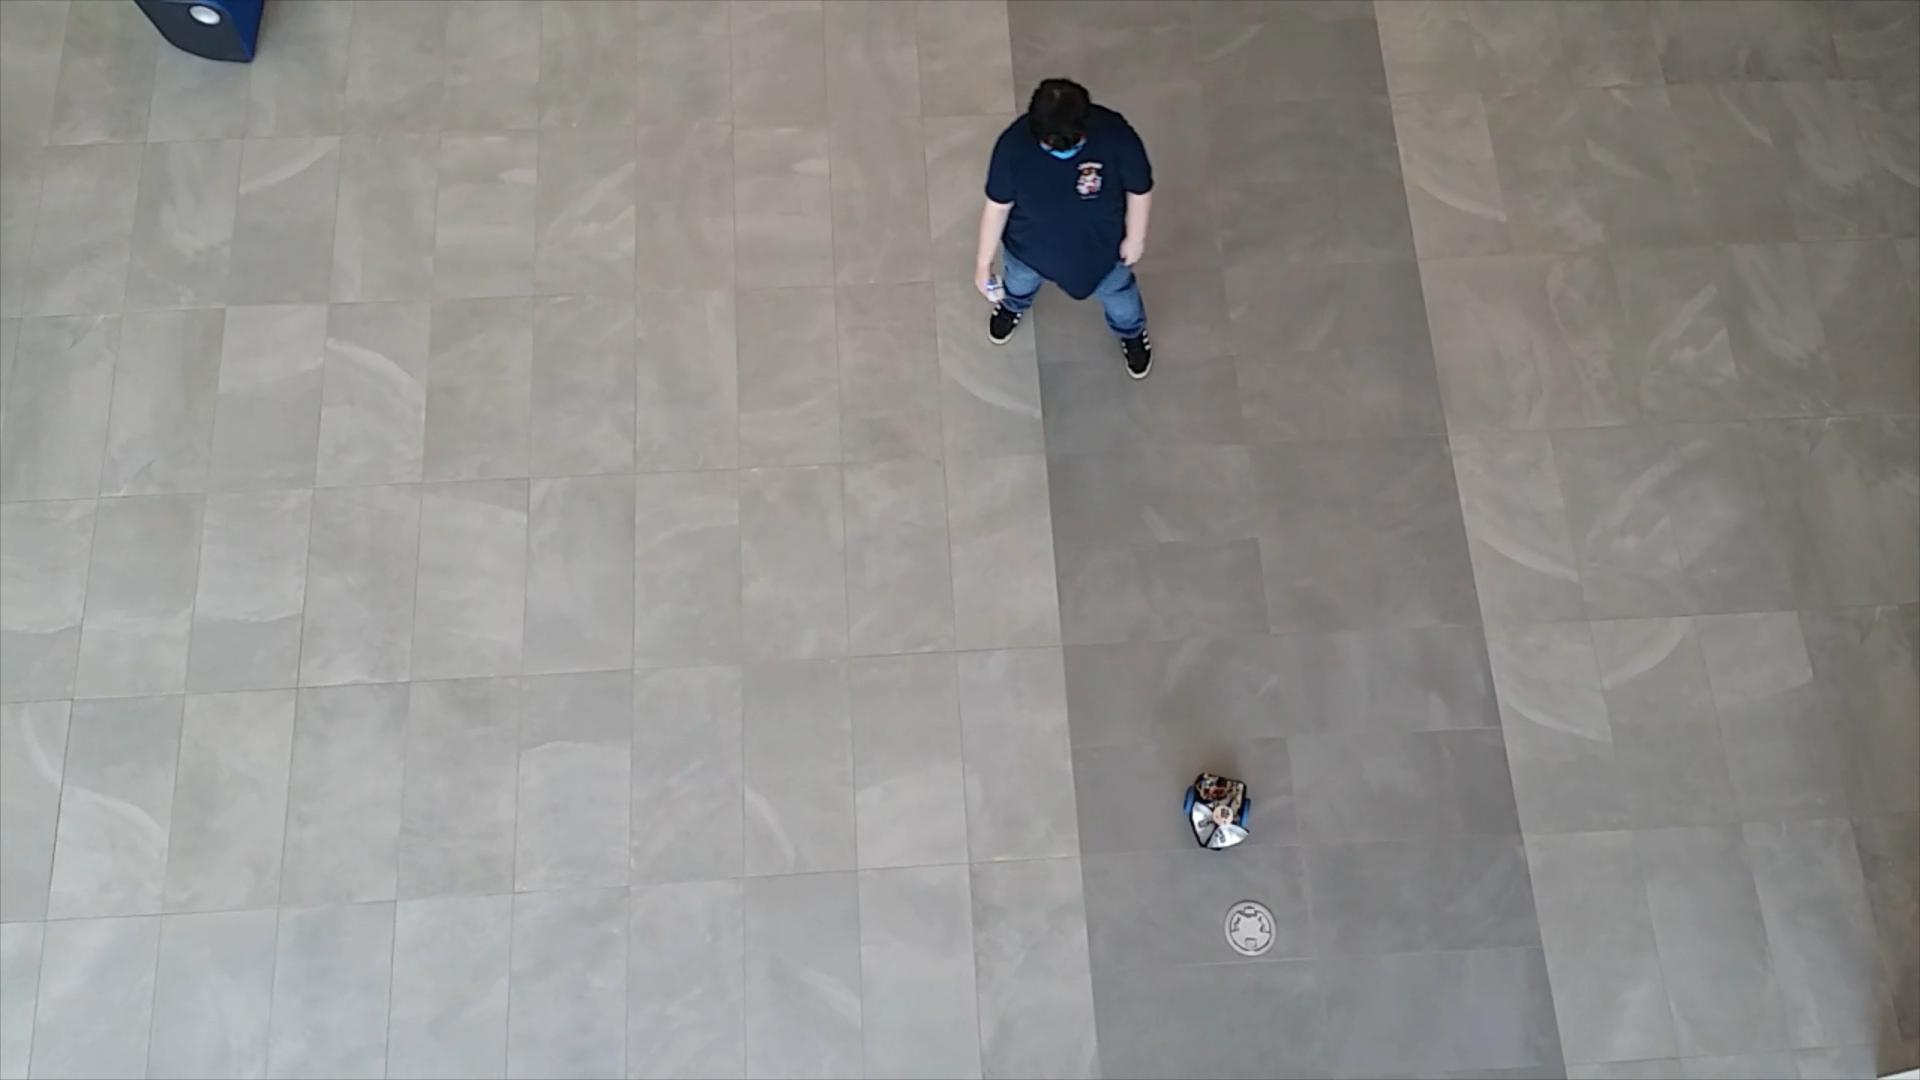
\includegraphics[width=\textwidth]{videos/frames/561.jpeg} 
    \caption{}
    \label{fig:561}
  \end{subfigure}
  %
  \\
  \begin{subfigure}[b]{0.30\linewidth}
    \centering
    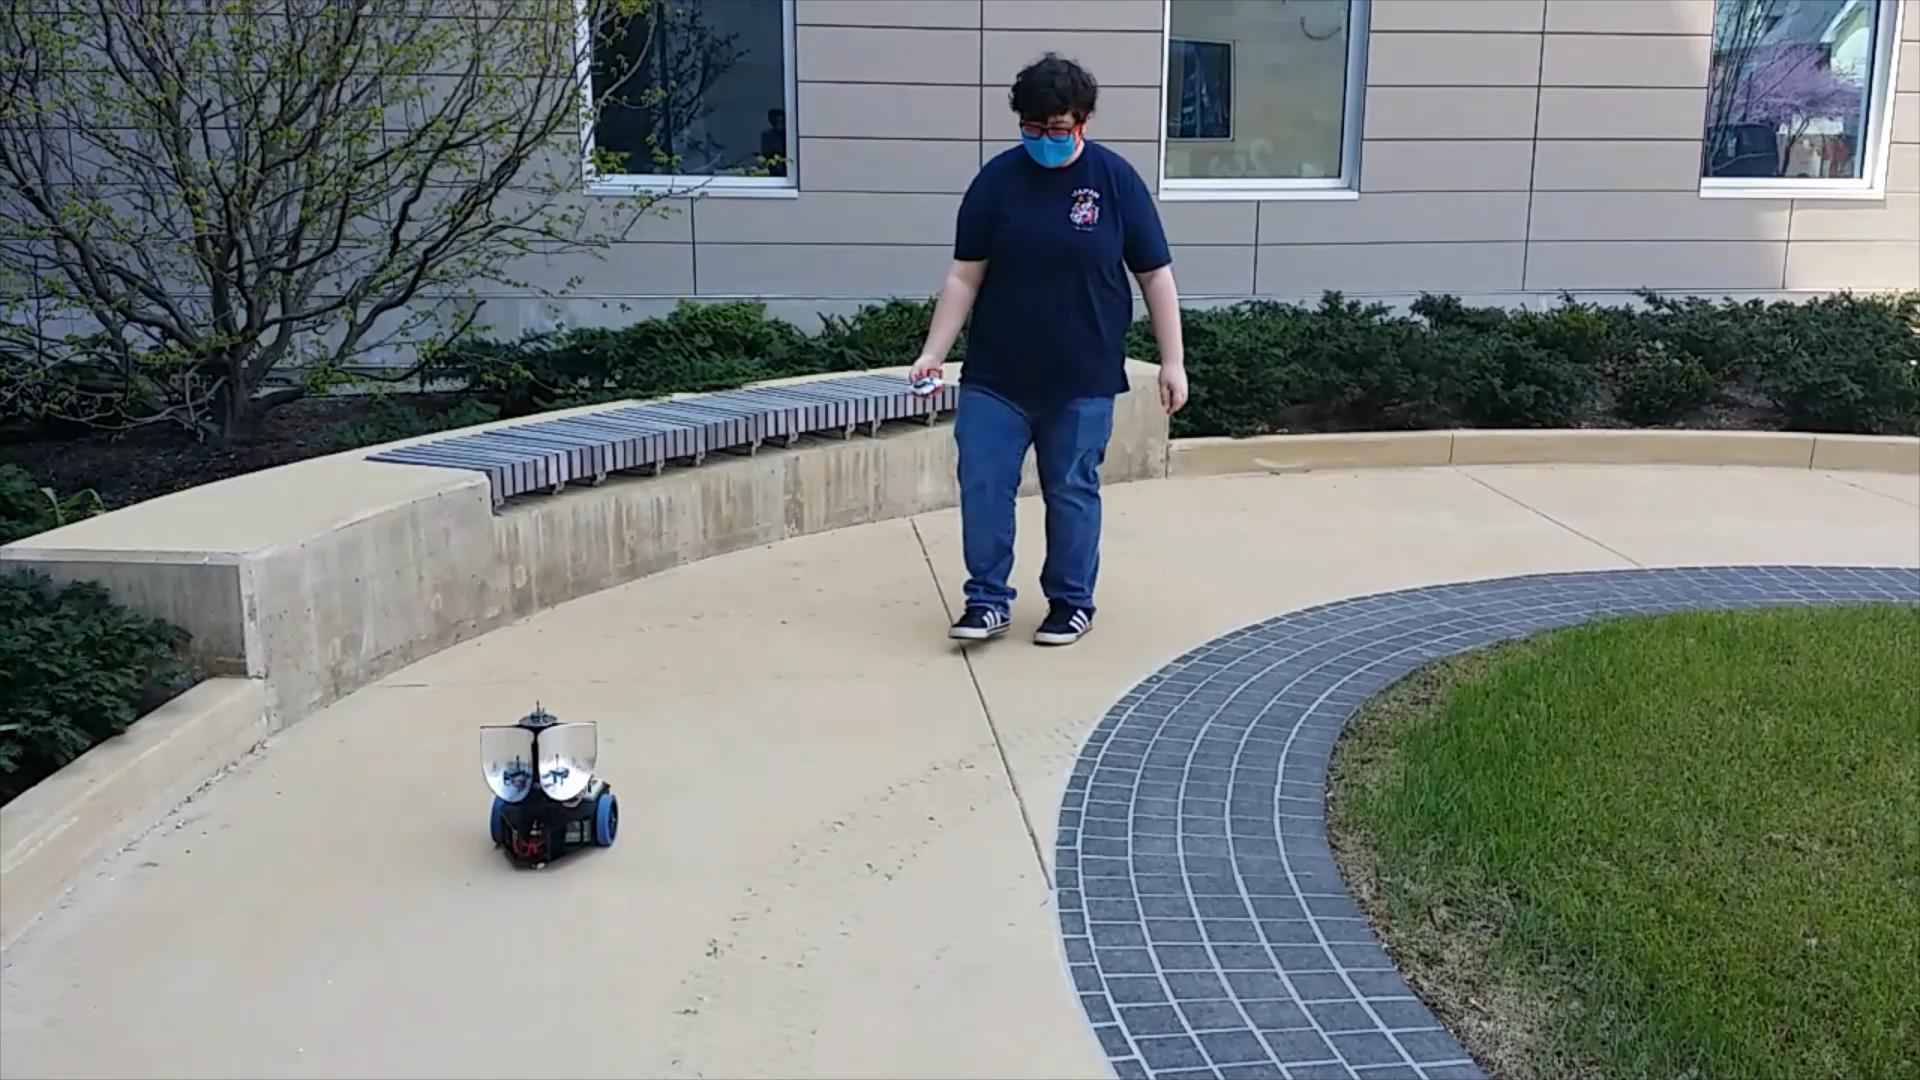
\includegraphics[width=\textwidth]{videos/frames/631.jpeg} 
    \caption{}
    \label{fig:631}
  \end{subfigure}
  %
  \begin{subfigure}[b]{0.30\linewidth}
    \centering
    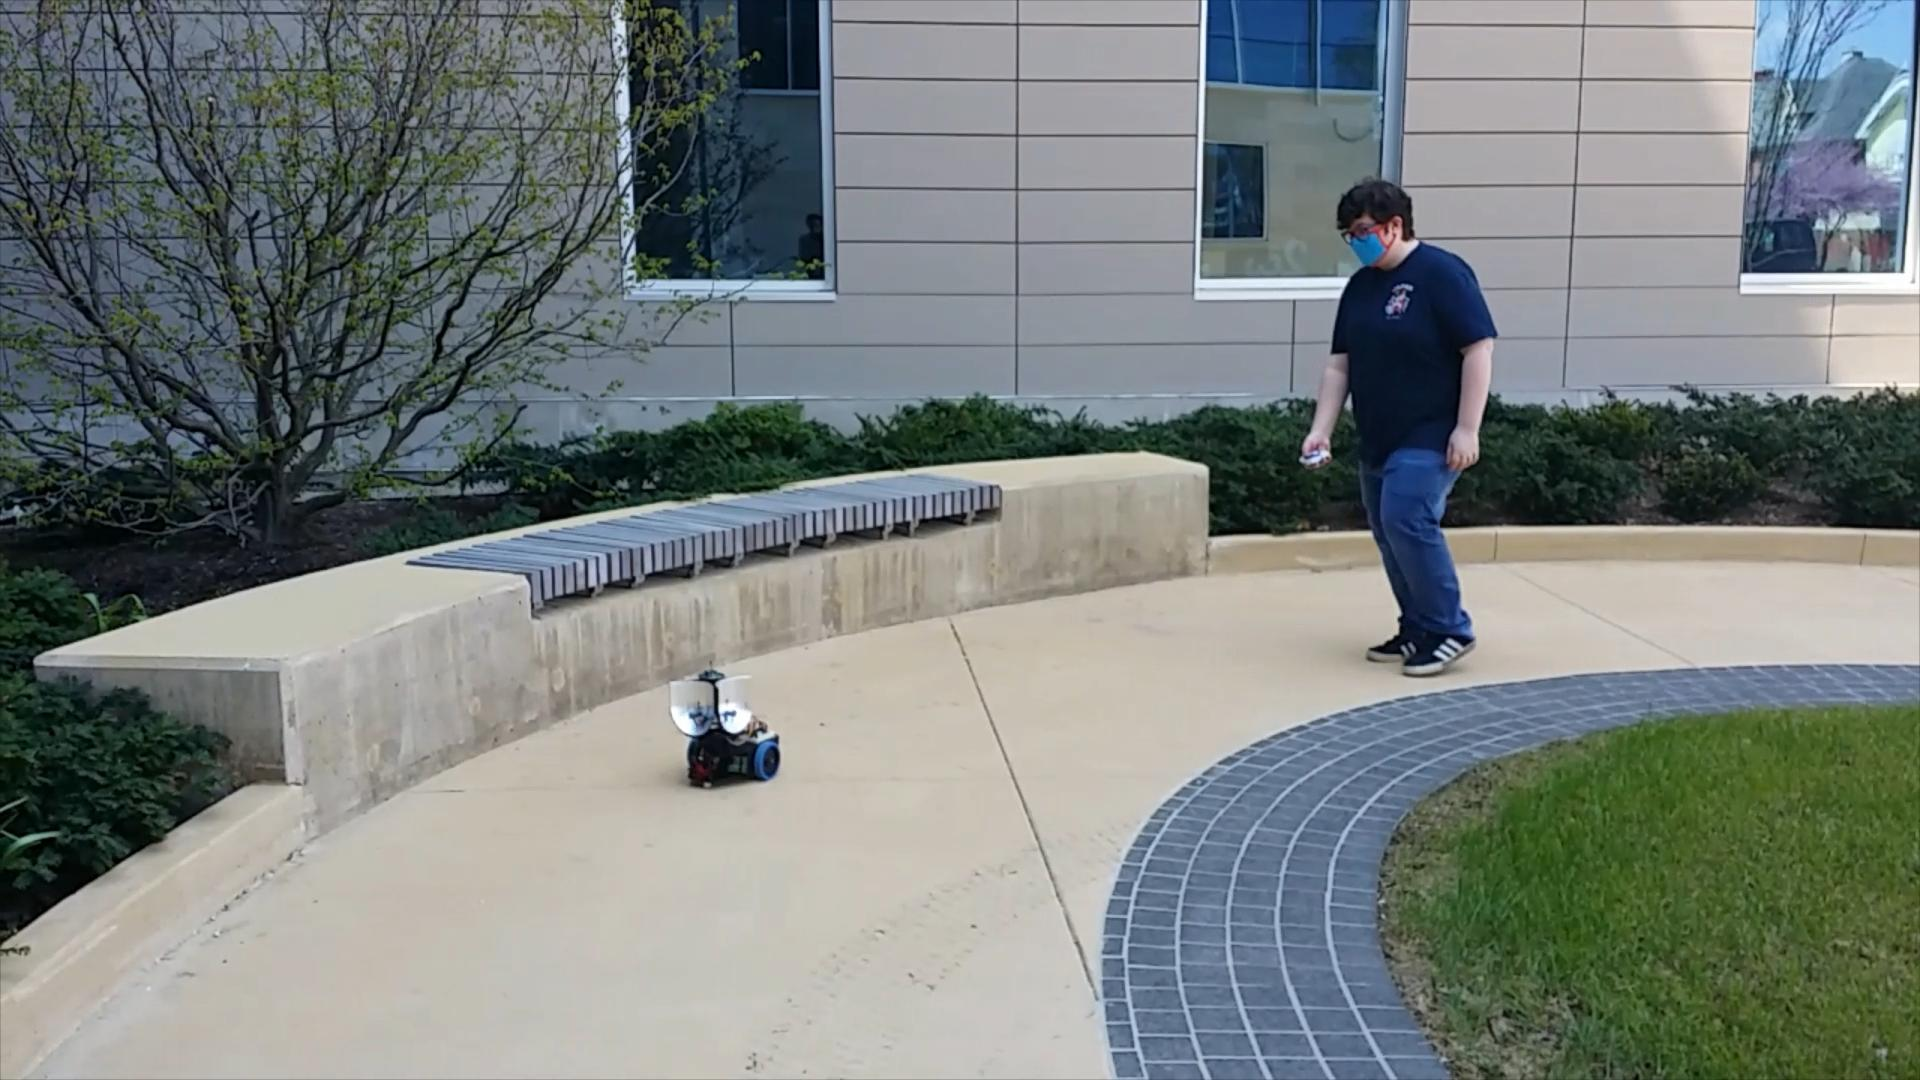
\includegraphics[width=\textwidth]{videos/frames/701.jpeg} 
    \caption{}
    \label{fig:701}
  \end{subfigure}
  %
  \caption{Experiment results demonstrating the performance of the proposed smart robotic cart in following the remote.}
  \label{fig:experResultsImages}
\end{figure}
%
Fig.~\ref{fig:experResultsImages} summarizes the performance of the proposed smart robotic cart. A person holding the remote shown in Fig.~\ref{fig:remotePrototype} follows a random trajectory. As can be seen, the mobile cart shown in Fig.~\ref{fig:overallPrototype} is able to follow the remote regardless of the navigation environment of both of the remote and the mobile cart. 



%----------------------------------------------------------------------
\section{Conclusion and Future Work}
%----------------------------------------------------------------------
In this paper, we have presented a prototype of a smart robotic cart using radio
frequency signal strengths. In the proposed smart robotic cart, the mobile cart
follows a remote. A functional design for a mobile cart was developed and
tested. In these tests, it was concluded that with the robot's current design,
it would be extremely difficult to calculate an accurate distance to the remote
from the signal strength alone. Therefore, the current design follows the remote
based on angle measurements alone. Due to the limitation of not having a proper
estimated line-of-sight distance, the current implementation is unable to
dynamically adjust its behavior based on proximity to the remote. One such
planned parameter was the robot's velocity, which would have been reduced as the
robot approached the remote target to prevent it from running into the user.


Based on the literature review, it was determined that the smart robotic cart
design of this cart is more cost-effective than most, if not all, of the
existing solutions. It was shown that the robot could successfully track the
remote target even when obstacles were obstructing the line-of-sight path
between the robot and remote. An immediate future research avenue of this work
is to implement filtering algorithms for estimating line-of-sight distance
between the mobile cart and the remote.

\bibliographystyle{IEEEtran}
\bibliography{bib/references.bib}

\end{document}
